\documentclass[12pt,a4paper,titlepage]{article}
\usepackage[utf8]{inputenc}
\usepackage{polski}
\usepackage[margin=1in]{geometry}
\usepackage{listings}
\usepackage{graphicx}
\usepackage{xcolor}
\usepackage{minted}
\usepackage{multirow}
\usepackage{longtable}
\usepackage{ctable}
\usepackage{float}
\usepackage{tabu}
\usepackage{longtable}
\usepackage{url}

\usepackage{caption} 
\captionsetup[table]{skip=10pt}

\newcommand{\specialcell}[2][c]{
  \begin{tabular}[#1]{@{}c@{}}#2\end{tabular}
}
\newcommand{\specialcellbold}[2][c]{
  \bfseries
  \begin{tabular}[#1]{@{}c@{}}#2\end{tabular}
}

\PassOptionsToPackage{hyphens}{url}\usepackage{hyperref}
  
\makeatletter
\newcommand{\linia}{\rule{\linewidth}{0.4mm}}
\renewcommand{\maketitle}{\begin{titlepage}
    \vspace*{1cm}
    \begin{center}\small
    Politechnika Wrocławska\\
    Wydział Elektroniki\\
    Technologie Sieciowe
    \end{center}
    \vspace{3cm}
    \noindent\linia
    \begin{center}
      \LARGE \textsc{\@title}
         \end{center}
     \linia
    \vspace{0.5cm}
    \begin{flushright}
    \begin{minipage}{7cm}
    \textit{\small Autorzy:}\\
    \normalsize \textsc{\@author} \par
    \end{minipage}
    \vspace{5cm}

     {\small wtorek, 17\textsuperscript{05}-18\textsuperscript{45} TN}\\
        Dr inż. Michał Kucharzak
     \end{flushright}
    \vspace*{\stretch{6}}
    \begin{center}
    \today
    \end{center}
  \end{titlepage}%
}
\makeatother
\author{Justyna Skalska, 225942 \\
Bartosz Powęska, 234720
}
\title{Projekt sieci}

\begin{document}
\maketitle
\tableofcontents
\newpage
\section{Wstęp}
Niniejsza dokumentacja jest projektem lokalnej sieci komputerowej dla firmy „G.I. Industries” zajmującej się produkcją oprogramowania znajdującego zastosowanie w obsłudze specjalistycznych robotów używanych w procesie produkcji pojazdów militarnych. Projekt został opracowany na podstawie dokumentacji dostarczonej przez zleceniodawcę i jest przystosowany na przewidywany wzrost liczby pracowników. W pracach nad projektem kierowano się przede wszystkim niezawodnością (przy przewidywanych obciążeniach) i łatwością rozbudowy sieci w przyszłości.
\section{Inwentaryzacja zasobów}

Siedziba firmy składa się z dwóch znajdujących się blisko siebie budynków. Pierwszy budynek jest dwupiętrowy, drugi natomiast jest parterowcem. Pomiędzy nimi nie znajdują się żadne zabudowania. W firmie są trzy grupy robocze: zarząd i kadry, programiści i testerzy oraz administratorzy.

\begin{table}[H]
    \centering
    \caption{Podstawowa inwentaryzacja zasobów przedsiębiorstwa}
    \begin{tabular}{c|c|c|c|c|}
    \cline{2-5}
    & \multicolumn{4}{c|}{\specialcellbold{Liczba użytkowników}} \\ \cline{2-5}
    & \multicolumn{3}{c|}{\specialcellbold{Budynek A}} & \multicolumn{1}{c|}{\specialcellbold{Budynek B}} \\ \hline 
         \multicolumn{1}{|c|}{\specialcellbold{Grupa robocza}} & \specialcellbold{Parter} & \specialcellbold{Piętro 1} & \specialcellbold{Piętro 2} & \specialcellbold{Parter} \\ \hline
         \multicolumn{1}{|c|}{Zarząd i kadry} & - & 6 & 16 & 12 \\ \hline
         \multicolumn{1}{|c|}{Programiści i testerzy} & - & 49 & 31 & 68 \\ \hline
         \multicolumn{1}{|c|}{Administratorzy} & 4 & - & - & 2 \\ \hline
         & \multicolumn{4}{c|}{\specialcellbold{Liczba drukarek}} \\ \cline{2-5}
         & 1 & 2 & 2 & 2 \\ \cline{2-5}
         & \multicolumn{4}{c|}{\specialcellbold{Kamery IP}} \\ \cline{2-5}
         & 8 & 5 & 5 & 8 \\ \cline{2-5}
         & \multicolumn{4}{c|}{\specialcellbold{Laboratorium}} \\ \cline{2-5}
         & 16 & - & - & - \\ \cline{2-5}
    \end{tabular}
    \label{tab:inwentaryzacja_zasobow}
\end{table}

\begin{table}[H]
    \centering
    \caption{Obecne zasoby firmy}
    \begin{tabular}{|c|c|} \hline
         \specialcellbold{Rodzaj zasobu} & \specialcellbold{Liczba} \\ \hline
         Komputer & 188 \\ \hline
         Drukarka & 7 \\ \hline
         Kamery IP & 26 \\ \hline
         Roboty & 16 \\ \hline 
    \end{tabular}
    \label{tab:zasoby_firmy}
\end{table}

\begin{table}[H]
    \centering
    \caption{Aplikacje wykorzystywane w firmie}
    \begin{tabular}{|c|c|} \hline
        \specialcellbold{Rodzaj programu} & \specialcellbold{Przykład} \\ \hline
        Przeglądarka internetowa & Mozilla Firefox, Google Chrome \\ \hline
        Komunikator & Discord, HipChat \\ \hline
        Klient FTP & FileZilla, Cyberduck \\ \hline
        VoIP & Discord, HipChat  \\ \hline
        Wideokonferencja & Zoom, Google Hangouts \\ \hline
    \end{tabular}
    \label{tab:aplikacje_w_firmie}
\end{table}

\begin{table}[H]
    \centering
    \caption{Punkty dystrybucyjne}
    \begin{tabular}{|c|c|c|} \hline
        \specialcellbold{Oznaczenie} & \specialcellbold{Lokalizacja} & \specialcellbold{Podłączone punkty abonencie} \\ \hline
        MDF  & Budynek A, Parter   & Budynek A, Parter \\ \hline
        IDF1 & Budynek A, Piętro 1 & Budynek A, Piętro 1 \\ \hline
        IDF2 & Budynek A, Piętro 2 & Budynek A, Piętro 2 \\ \hline
        IDF3 & Budynek B, Parter   & Budynek B \\ \hline
    \end{tabular}
    \label{tab:punkty_dystrybucyjne}
\end{table}

\section{Analiza potrzeb użytkowników}

\begin{table}
    \centering
    \caption{Przepływ danych jednego użytkownika z/do Internetu}
    \begin{tabular}{c|c|c|c|c|} \cline{2-5}
        & \multicolumn{4}{c|}{\specialcellbold{Transfer (down/up), kb/s}} \\ \hline
        \multicolumn{1}{|c|}{\specialcellbold{Użytkownik/\\Aplikacja}} & \specialcellbold{Przeglądarka} & \specialcellbold{Praca w \\ chmurze} & \specialcellbold{Komunikator} & \specialcellbold{Wideorozmowy} \\ \hline
        \multicolumn{1}{|c|}{Zarząd i kadry} & 80/15 & 23/36 & 15/15 & 40/40 \\ \hline
        \multicolumn{1}{|c|}{\specialcell{Programiści \\i testerzy}} & 110/10 & 30/53 & 15/15 & 40/40 \\ \hline
        \multicolumn{1}{|c|}{Administratorzy} & 100/20 & 20/30 & 15/15 & 10/10 \\ \hline
        \multicolumn{1}{|c|}{Sieć gości} & 20/10 & 5/5 & 5/5 & - \\ \hline
    \end{tabular}
    \label{tab:transfer_osoba_internet}
\end{table}

\begin{table}[H]
    \centering
    \caption{Transfer danych z/do Internetu}
    \begin{tabular}{|c|c|c|c|c|c|c|} \hline
        \multirow{3}{*}{\specialcellbold{Punkt\\dystrybucyjny}} & \multicolumn{2}{c|}{\specialcellbold{Grupa robocza}} & \multicolumn{4}{c|}{\specialcellbold{Internet (kb/s)}} \\ \cline{2-7}
        & \specialcellbold{Nazwa} & \specialcellbold{Liczba\\stanowisk} & DOWN & UP & \specialcell{UP\\łącznie} & \specialcell{DOWN\\łącznie} \\ \hline
        \multirow{5}{*}{MDF}
        & Zarząd i kadry                        & - & 158 & 106 &   - &   - \\ \cline{2-7}
        & \specialcell{Programiści\\i testerzy} & - & 195 & 118 &   - &   - \\ \cline{2-7}
        & Administratorzy                       & 4 & 145 &  75 & 580 & 300 \\ \cline{2-7}
        & Sieć gości                            & - &  30 &  20 &   - &   - \\ \cline{2-7}
        & Łącznie                               & 4 & - & - & 580 & 300 \\ \hline
        
        \multirow{5}{*}{IDF1}
        & Zarząd i kadry                        & 16 & 158 & 106 & 2528 & 1696 \\ \cline{2-7}
        & \specialcell{Programiści\\i testerzy} & 31 & 195 & 118 & 6045 & 3658 \\ \cline{2-7}
        & Administratorzy                       & - & 145 & 75 & - & - \\ \cline{2-7}
        & Sieć gości                            & - & 30 & 20 & - & - \\ \cline{2-7}
        & Łącznie                               & 47 & - & - & 8573 & 5354 \\ \hline
        
        \multirow{5}{*}{IDF2}
        & Zarząd i kadry                        & 6 & 158 & 106 & 948 & 636 \\ \cline{2-7}
        & \specialcell{Programiści\\i testerzy} & 49 & 195 & 118 & 9555 & 5782 \\ \cline{2-7}
        & Administratorzy                       & - & 145 & 75 & - & - \\ \cline{2-7}
        & Sieć gości                            & - & 30 & 20 & - & - \\ \cline{2-7}
        & Łącznie                               & 55 & - & - & 10503 & 6418 \\ \hline
        
        \multirow{5}{*}{IDF3}
        & Zarząd i kadry                        & 12 & 158 & 106 & 1896 & 1272 \\ \cline{2-7}
        & \specialcell{Programiści\\i testerzy} & 68 & 195 & 118 & 13260 & 8024 \\ \cline{2-7}
        & Administratorzy                       & 2 & 145 & 75 & 290 & 150 \\ \cline{2-7}
        & Sieć gości                            & - & 30 & 20 & - & - \\ \cline{2-7}
        & Łącznie                               & 82 & - & - & 15446 & 9446 \\ \hline
        
        \multirow{1}{*}{Łącznie}                
        & -                                     & 188 & - & - & 35102 & 21518 \\ \hline
    \end{tabular}
    \label{tab:transfer_internet}
\end{table}

\begin{table}[H]
    \centering
    \caption{Transfer danych z/do serwera plików 1}
    \begin{tabular}{|c|c|c|c|c|c|c|} \hline
        \multirow{3}{*}{\specialcellbold{Punkt\\dystrybucyjny}} & \multicolumn{2}{c|}{\specialcellbold{Grupa robocza}} & \multicolumn{4}{c|}{\specialcellbold{Serwer plików 1 (kb/s)}} \\ \cline{2-7}
        & \specialcellbold{Nazwa} & \specialcellbold{Liczba\\stanowisk} & DOWN & UP & \specialcell{UP\\łącznie} & \specialcell{DOWN\\łącznie} \\ \hline
        \multirow{2}{*}{MDF}
        & Administratorzy   &  4 & 8000 &  600 & 32000 &  2400 \\ \cline{2-7}
        & Kamery            &  8 &  110 & 2800 &   880 & 22400 \\ \cline{2-7}
        & Łącznie           & 12 & - & - & 32880 & 24800 \\ \hline
        
        \multirow{2}{*}{IDF1}
        & Administratorzy   & - & 8000 &  600 &   - &     - \\ \cline{2-7}
        & Kamery            & 5 &  110 & 2800 & 550 & 14000 \\ \cline{2-7}
        & Łącznie           & 5 & - & - & 550 & 14000 \\ \hline
        
        \multirow{2}{*}{IDF2}
        & Administratorzy   & - & 8000 &  600 &   - &     - \\ \cline{2-7}
        & Kamery            & 5 &  110 & 2800 & 550 & 14000 \\ \cline{2-7}
        & Łącznie           & 5 & - & - & 550 & 14000 \\ \hline
        
        \multirow{2}{*}{IDF3}
        & Administratorzy   & 2 & 8000 &  600 & 16000 &  1200 \\ \cline{2-7}
        & Kamery            & 8 &  110 & 2800 &   880 & 22400 \\ \cline{2-7}
        & Łącznie           & 10 & - & - & 16880 & 23400 \\ \hline
        
        \multirow{1}{*}{Łącznie} 
        & -                 & 32 & - & - & 50860 & 76200 \\ \hline

    \end{tabular}
    \label{tab:transfer_serwer_1}
\end{table}

\begin{table}[H]
    \centering
    \caption{Transfer danych z/do serwera plików 2}
    \begin{tabular}{|c|c|c|c|c|c|c|} \hline
        \multirow{3}{*}{\specialcellbold{Punkt\\dystrybucyjny}} & \multicolumn{2}{c|}{\specialcellbold{Grupa robocza}} & \multicolumn{4}{c|}{\specialcellbold{Serwer plików 2 (kb/s)}} \\ \cline{2-7}
        & \specialcellbold{Nazwa} & \specialcellbold{Liczba\\stanowisk} & DOWN & UP & \specialcell{UP\\łącznie} & \specialcell{DOWN\\łącznie} \\ \hline
        
        \multirow{4}{*}{MDF}
        & Zarząd i kadry                            & - & 600 & 550 &    - &    - \\ \cline{2-7}
        & \specialcell{Programiści\\i testerzy}     & - & 700 & 590 &    - &    - \\ \cline{2-7}
        & Administratorzy                           & 4 & 800 & 300 & 3200 & 1200 \\ \cline{2-7}
        & Łącznie                                   & 4 & 800 & 300 & 3200 & 1200 \\ \hline
        
        \multirow{4}{*}{IDF1}
        & Zarząd i kadry                            &  6 & 600 & 550 &  3600 &  3300 \\ \cline{2-7}
        & \specialcell{Programiści\\i testerzy}     & 49 & 700 & 590 & 34300 & 28910 \\ \cline{2-7}
        & Administratorzy                           &  - & 800 & 300 &     - &     - \\ \cline{2-7}
        & Łącznie                                   & 55 &   - &   - & 37900 & 32210 \\ \hline
        
        \multirow{4}{*}{IDF2}
        & Zarząd i kadry                            & 16 & 600 & 550 &  9600 &  8800 \\ \cline{2-7}
        & \specialcell{Programiści\\i testerzy}     & 31 & 700 & 590 & 21700 & 18290 \\ \cline{2-7}
        & Administratorzy                           &  - & 800 & 300 &     -  &     - \\ \cline{2-7}
        & Łącznie                                   & 47 &   - &   - & 31300 & 27090 \\ \hline
        
        \multirow{4}{*}{IDF3}
        & Zarząd i kadry                            & 12 & 600 & 550 &  7200 &  6600 \\ \cline{2-7}
        & \specialcell{Programiści\\i testerzy}     & 68 & 700 & 590 & 47600 & 40120 \\ \cline{2-7}
        & Administratorzy                           & 2  & 800 & 300 &  1600 &   600 \\ \cline{2-7}
        & Łącznie                                   & 82 & -   & -   & 56400 & 47320 \\ \hline

        \multirow{1}{*}{Łącznie} 
        & -                                         & 188 & - & - & 128800 & 107820 \\ \hline      
    \end{tabular}
    \label{tab:transfer_serwer_2}
\end{table}

\begin{table}[H]
    \centering
    \caption{Transfer danych z/do serwera WWW}
    \begin{tabular}{|c|c|c|c|c|c|c|} \hline
        \multirow{3}{*}{\specialcellbold{Punkt\\dystrybucyjny}} & \multicolumn{2}{c|}{\specialcellbold{Grupa robocza}} & \multicolumn{4}{c|}{\specialcellbold{Serwer WWW (kb/s)}} \\ \cline{2-7}
        & \specialcellbold{Nazwa} & \specialcellbold{Liczba\\stanowisk} & DOWN & UP & \specialcell{UP\\łącznie} & \specialcell{DOWN\\łącznie} \\ \hline
        
        \multirow{4}{*}{MDF}
        & Zarząd i kadry                            & - & 330 & 440 &   - &   - \\ \cline{2-7}
        & \specialcell{Programiści\\i testerzy}     & - & 380 & 430 &   - &   - \\ \cline{2-7}
        & Administratorzy                           & 4 & 380 & 390 & 1520 & 1560 \\ \cline{2-7}
        & Łącznie                                   & 4 &   - &   - & 1520 & 1560 \\ \hline
        
        \multirow{4}{*}{IDF1}
        & Zarząd i kadry                            &  6 & 230 &  45 &  1380 &  270 \\ \cline{2-7}
        & \specialcell{Programiści\\i testerzy}     & 49 & 190 &  35 &  9310 & 1715 \\ \cline{2-7}
        & Administratorzy                           &  - & 210 &  60 &     - &    - \\ \cline{2-7}
        & Łącznie                                   & 55 &   - &   - & 10690 & 1985 \\ \hline
        
        \multirow{4}{*}{IDF2}
        & Zarząd i kadry                            & 16 & 230 &  45 &  5280 &  7040 \\ \cline{2-7}
        & \specialcell{Programiści\\i testerzy}     & 31 & 190 &  35 & 11780 & 13330 \\ \cline{2-7}
        & Administratorzy                           &  - & 210 &  60 &     - &     - \\ \cline{2-7}
        & Łącznie                                   & 47 &   - &   - & 17060 & 20370 \\ \hline
        
        \multirow{4}{*}{IDF3}
        & Zarząd i kadry                            & 12 & 230 &  45 &  3960 &  5280 \\ \cline{2-7}
        & \specialcell{Programiści\\i testerzy}     & 68 & 190 &  35 & 25840 & 29240 \\ \cline{2-7}
        & Administratorzy                           &  2 & 210 &  60 &   760 &   780 \\ \cline{2-7}
        & Łącznie                                   & 82 &   - &   - & 30560 & 35300 \\ \hline
        
        \multirow{1}{*}{Łącznie} 
        & -                                         & 188 & - & - & 59830 & 59215 \\ \hline 
    \end{tabular}
    \label{tab:transfer_serwer_www}
\end{table}

\begin{table}[H]
    \centering
    \caption{Transfer danych z/do serwera pocztowego}
    \begin{tabular}{|c|c|c|c|c|c|c|} \hline
        \multirow{3}{*}{\specialcellbold{Punkt\\dystrybucyjny}} & \multicolumn{2}{c|}{\specialcellbold{Grupa robocza}} & \multicolumn{4}{c|}{\specialcellbold{Serwer pocztowy (kb/s)}} \\ \cline{2-7}
        & \specialcellbold{Nazwa} & \specialcellbold{Liczba\\stanowisk} & DOWN & UP & \specialcell{UP\\łącznie} & \specialcell{DOWN\\łącznie} \\ \hline
        
        \multirow{4}{*}{MDF}
        & Zarząd i kadry                            & - & 230 &  45 &   - &   - \\ \cline{2-7}
        & \specialcell{Programiści\\i testerzy}     & - & 190 &  35 &   - &   - \\ \cline{2-7}
        & Administratorzy                           & 4 & 210 &  60 & 840 & 240 \\ \cline{2-7}
        & Łącznie                                   & 4 &   - &   - & 840 & 240 \\ \hline
        
        \multirow{4}{*}{IDF1}
        & Zarząd i kadry                            &  6 & 230 &  45 &  1380 &  270 \\ \cline{2-7}
        & \specialcell{Programiści\\i testerzy}     & 49 & 190 &  35 &  9310 & 1715 \\ \cline{2-7}
        & Administratorzy                           &  - & 210 &  60 &     - &    - \\ \cline{2-7}
        & Łącznie                                   & 55 &   - &   - & 10690 & 1985 \\ \hline
        
        \multirow{4}{*}{IDF2}
        & Zarząd i kadry                            & 16 & 230 &  45 & 3680 &  720 \\ \cline{2-7}
        & \specialcell{Programiści\\i testerzy}     & 31 & 190 &  35 & 5890 & 1085 \\ \cline{2-7}
        & Administratorzy                           &  - & 210 &  60 &    - &    - \\ \cline{2-7}
        & Łącznie                                   & 47 &   - &   - & 9570 & 1805 \\ \hline
        
        \multirow{4}{*}{IDF3}
        & Zarząd i kadry                            & 12 & 230 &  45 &  2760 &  540 \\ \cline{2-7}
        & \specialcell{Programiści\\i testerzy}     & 68 & 190 &  35 & 12920 & 2380 \\ \cline{2-7}
        & Administratorzy                           &  2 & 210 &  60 &   420 &  120 \\ \cline{2-7}
        & Łącznie                                   & 82 &   - &   - & 16100 & 3040 \\ \hline
        
        \multirow{1}{*}{Łącznie} 
        & -                                         & 188 & - & - & 96415 & 7070 \\ \hline 
    \end{tabular}
    \label{tab:transfer_serwer_pocztowy}
\end{table}

\begin{table}[H]
    \centering
    \caption{Transfer danych z/do drukarki}
    \begin{tabular}{|c|c|c|c|c|c|c|} \hline
        \multirow{3}{*}{\specialcellbold{Punkt\\dystrybucyjny}} & \multicolumn{2}{c|}{\specialcellbold{Grupa robocza}} & \multicolumn{4}{c|}{\specialcellbold{Drukarka (kb/s)}} \\ \cline{2-7}
        & \specialcellbold{Nazwa} & \specialcellbold{Liczba\\stanowisk} & DOWN & UP & \specialcell{UP\\łącznie} & \specialcell{DOWN\\łącznie} \\ \hline
        
        \multirow{4}{*}{MDF}
        & Zarząd i kadry                            & - & 10 &  180 &  - &   - \\ \cline{2-7}
        & \specialcell{Programiści\\i testerzy}     & - & 10 &  170 &  - &   - \\ \cline{2-7}
        & Administratorzy                           & 4 & 10 &  175 & 40 & 700 \\ \cline{2-7}
        & Łącznie                                   & 4 &  - &    - & 40 & 700 \\ \hline
        
        \multirow{4}{*}{IDF1}
        & Zarząd i kadry                            &  6 & 10 &  180 &  60 & 1080 \\ \cline{2-7}
        & \specialcell{Programiści\\i testerzy}     & 49 & 10 &  170 & 490 & 8330 \\ \cline{2-7}
        & Administratorzy                           &  - & 10 &  175 &   - &    - \\ \cline{2-7}
        & Łącznie                                   & 55 &   - &   - & 550 & 9410 \\ \hline
        
        \multirow{4}{*}{IDF2}
        & Zarząd i kadry                            & 16 & 10 &  180 & 160 & 2880 \\ \cline{2-7}
        & \specialcell{Programiści\\i testerzy}     & 31 & 10 &  170 & 310 & 5270 \\ \cline{2-7}
        & Administratorzy                           &  - & 10 &  175 &   - &    - \\ \cline{2-7}
        & Łącznie                                   & 47 &   - &   - & 470 & 8150 \\ \hline
        
        \multirow{4}{*}{IDF3}
        & Zarząd i kadry                            & 12 & 10 & 180 & 120 &  2160 \\ \cline{2-7}
        & \specialcell{Programiści\\i testerzy}     & 68 & 10 & 170 & 680 & 11560 \\ \cline{2-7}
        & Administratorzy                           &  2 & 10 & 175 &  20 &   350 \\ \cline{2-7}
        & Łącznie                                   & 82 &  - &   - & 820 & 14070 \\ \hline
        
        \multirow{1}{*}{Łącznie} 
        & -                                         & 188 & - & - & 1880 & 32330 \\ \hline 
    \end{tabular}
    \label{tab:transfer_drukarka}
\end{table}

\begin{table}[H]
    \centering
    \caption{Transfer danych pomiędzy serwerami i Internetem}
    \begin{tabular}{c|c|c|c|} \cline{2-3}
        & \multicolumn{2}{c|}{\specialcellbold{Internet (kb/s)}} \\ \cline{2-4}
        & \specialcellbold{Down} & \specialcellbold{Up} & \specialcellbold{Sesje} \\ \hline
        \multicolumn{1}{|c|}{Serwer WWW}      &  80 & 170 & 96 \\ \hline
        \multicolumn{1}{|c|}{Serwer pocztowy} & 890 & 410 & 12 \\ \hline
    \end{tabular}
    \label{tab:transfer_internet_serwery}
\end{table}

\begin{table}[H]
    \centering
    \caption{Transfer danych pomiędzy sieciami laboratoryjną i biurową}
    \begin{tabular}{|c|c|} \hline
        \multicolumn{2}{|c|}{\specialcellbold{Transfer danych (kb/s)}} \\ \hline
        \specialcellbold{Down} & \specialcellbold{Up} \\ \hline
        27200 & 27200 \\ \hline
    \end{tabular}
    \label{tab:transfer_lab_biuro}
\end{table}

\section{Założenia projektowe}
Założenia projektowe obejmują wdrożenie sieci w siedzibie firmy "G.I. Industries", która mieści się w dwóch budynkach połączonych kablem światłowodowym. Sieć będzie nowoczesna i łatwa w rozbudowie. W budynkach należących do przedsiębiorstwa zostało zainstalowane okablowanie strukturalne (kat.  6) wraz z niezbędnymi szafami teleinformatycznymi oraz wszystkie  urządzenia  końcowe (serwery,  drukarki, komputery,  kamery  IP,  itp.), które należy podłączyć do sieci.
W budynkach znajdują się cztery punkty dystrybucyjne z szafami teleinformatycznymi, do których schodzą się kable z obsługiwanych przez nie gniazd z różnych pięter i budynków. Odległość pomiędzy punktem dystrybucyjnym MDF a punktami IDF w każdym budynku nie przekracza 90 metrów,  pomiędzy  MDF  a  wszystkimi  IDF  w  obrębie  każdego  budynku  zainstalowano  okablowanie miedziane (skrętka) kat. 6.
\begin{itemize}
    \item MDF - główny punkt dystrybucyjny zlokalizowany na parterze budynku A obsługuje ruch generowany przez 4 użytkowników,
    \item IDF1 - pomocniczy punkt dystrybucyjny zlokalizowany na pierwszym piętrze budynku A obsługuje ruch generowany przez 55 użytkowników,
    \item IDF2 - pomocniczy punkt dystrybucyjny znajdujący się na drugim piętrze budynku A obsługujący 47 użytkowników
    \item IDF3 - pomocniczy punkt dystrybucyjny zlokalizowany na parterze budynku B obsługujący 82 użytkowników
\end{itemize}
Użytkownicy podzieleni są na 3 grupy robocze: administratorzy, programiści i testerzy oraz zarząd i kadry.\bigskip\\
Do punktów dystrybucyjnych należy także sprzęt należący do klienta:
\begin{itemize}
    \item serwer WWW,
    \item serwer pocztowy,
    \item serwer plików 1,
    \item serwer plików 2,
    \item 2 punkty dostępowe WiFi,
    \item 7 drukarek,
    \item 26 kamer IP,
    \item 16 robotów.
\end{itemize}
Konieczna jest instalacja i konfiguracja serwerów, przełączników, routera oraz punktów dostępowych.

Główne założenia projektowe:
\begin{itemize}
    \item Okablowanie poziome oraz szkieletowe znajdujące się wewnątrz budynków będzie wykonane w standardzie Gigabit Ethernet 1000Base-T (skrętka kat. 6),
    \item Połączenie między budynkami będzie wykorzystywało kable światłowodowe jednomodowe,
    \item Sieć będzie posiadać co najmniej 20\% wolnych portów na przełącznikach, aby umożliwić przyszłą rozbudowę spowodowaną wzrostem liczby pracowników,
    \item Technologia VLAN pozwoli na ograniczenie ilości burz broadcastowych, zwiększenie bezpieczeństwa sieci oraz umożliwi logiczne grupowanie stacji końcowych, które są fizycznie rozproszone w sieci
    \item Zapewnienie odpowiedniej konfiguracji sieci bezprzewodowej i kontroli dostępu poprzez usługę RADIUS oraz odseparowana sieci dla gości. Do szyfrowania sieci WiFi zostanie użyty standard szyfrowania WPA2-Enterprise,
    \item Niezawodność połączenia z internetem zostanie zapewniona dzięki dzierżawie łączy od dwóch niezależnych od siebie operatorów
    \item Serwery obsługujące ruch internetowy zostaną odizolowane w strefie DMZ, aby  w przypadku  włamania,  atakujący  nie  uzyskał  dostępu  do  całej  sieci komputerowej przedsiębiorstwa,
    \item Ochrona  przed  dostępem do wewnętrznych zasobów z zewnątrz zostanie osiągnięta poprzez prywatną adresację,
    \item Odporność na fizyczne uszkodzenia będzie zapewniony dzięki redundancji zasobów.
\end{itemize}

\section{Projekt sieci}
\subsection{Projekt logiczny sieci}

Ze względu na charakterystykę działania firmy sieć zostanie podzielona na VLAN-y odpowiadające
każdej grupie użytkowników pracujących w firmie. Pozwoli to na łatwe dołączanie osób do poszczególnych
grup.
Podział na VLAN-y:

\begin{itemize}
    \item VLAN777: Zarząd i kadry,
    \item VLAN888: Programiści i testerzy,
    \item VLAN999: Administratorzy,
    \item VLAN10: Sieć gości,
    \item VLAN20: Kamery,
    \item VLAN30: Drukarki,
    \item VLAN55: Serwery plików,
    \item VLAN66: DMZ,
    \item VLAN1000: Roboty,
    \item VLAN1001: Roboty (interfejs debugowania).
    \item VLAN5: Przełączniki dostępowe 
    \item VLAN6: Przełączniki szkieletowe 
\end{itemize}
Aby możliwy był dostęp do drukarek (VLAN30) oraz serwerów plików (VLAN55) z komputerów pracowników (VLAN777,VLAN888,VLAN999) na
przełącznikach warstwy 3 skonfigurowany zostanie InterVLAN Routing. Pozwoli on przekierować
ruch sieciowy z jednego VLANu do drugiego.
Koleją funkcją skonfigurowaną na przełącznikach warstwy 3 będzie Access Control List (ACL).
Listy kontroli dostępu pozwolą na ustalenie reguł przepływu ruchu między VLANami.

\begin{itemize}
    \item Ruch pomiędzy poszczególnymi grupami pracowników będzie blokowany (np. Programiści i testerzy nie uzyskają,
dostępu do urządzeń znajdujących się w VLANie zarządu i kadr),
    \item VLAN777,VLAN888,VLAN999 (Zarząd i kadry, programiści i testerzy, administratorzy) uzyskają dostęp do VLAN30 oraz VLAN55 (Drukarki, Serwery),
    \item VLAN10 (Sieć bezprzewodowa Wi-Fi) będzie mieć zablokowany dostęp do wszystkich innych VLANów,
    \item Dostęp do VLAN1000 i VLAN1001 (Laboratorium) będą mieć tylko programiści i testerzy (VLAN888).
\end{itemize}

Kluczowe dla działania sieci urządzenia (punkty dystrybucyjne) będą posiadały bliźniacze urządzenie
zapasowe. Punkty dystrybucyjne będą połączone w topologii siatki częściowej.

\begin{itemize}
    \item Główny punkt dystrybucyjny (MDF) oraz urządzenie zapasowe (MDF AUX) będą połączone za pomocą łącza światłowodowego z pośrednim punktem dystrybucyjnym (IDF3) znajdującym się w drugim budynku oraz jego urządzeniem zapasowym (IDF3 AUX).
    \item Punkty dystrybucyjne znajdujące się w w budynku A (MDF, IDF1, IDF2) oraz ich urządzenia zapasowe (MDF AUX, IDF1 AUX, IDF2 AUX) zostaną połączone za pomocą łącza Gigabit Ethernet,
\end{itemize}

Taka konfiguracja szkieletu sieci w razie prawidłowego działania urządzeń podstawowych pozwoli na rozkładanie się obciążenia w sieci. W przypadku IDF-ów w razie awarii któregoś urządzenia podstawowego jego funkcje przejmie urządzenie zapasowe. Jedynie w przypadku awarii dwóch urządzeń (podstawowego oraz zapasowego) określony fragment sieci przestanie działać. W przypadku MDF-a w razie awarii urządzenia podstawowego oraz zapasowego zostanie przerwana komunikacja między budynkami oraz utracony dostęp do sieci Internetowej. Jednak awaria obydwu urządzeń odpowiedzialnych za dany punkt dystrybucyjny to sytuacja niezwykle rzadka. Dodatkową zaletą takiej konfiguracji jest możliwość przeprowadzania prac konserwacyjnych bez zakłóceń działania sieci. Między przełącznikami warstwy trzeciej skonfigurowane zostanie funkcja EtherChannel, pozwalająca na połączenie kilku łączy fizycznych w jedno logiczne. Dzięki temu, przełączniki mogą równomiernie rozkładać obciążenie na łączu. Zapewni to wydajne połączenie między urządzeniami sieciowymi. Na każdym piętrze znajdował się będzie przełącznik warstwy drugiej podłączony do dwóch przełączników warstwy trzeciej (punkt dystrybucyjny oraz urządzenie zapasowe). W budynku drugim będą znajdować się dwa routery na których zostanie skonfigurowana obsługa protokołu VRRP. Pozwoli to na stworzenie klastra dostępowego (wirtualny router). Do każdego routera zostanie przypięte łącze Internetowe od niezależnego dostawcy (zapewni to redundancje połączenia z Internetem). Taka konfiguracja routerów przyspieszy to ruch sieciowy, zwiększy niezawodność oraz bezpieczeństwo. W sieci zostanie wydzielona strefa zdemilitaryzowana (DMZ). Strefa zdemilitaryzowana (ograniczonego zaufania) jest to wydzielony obszar nienależący do sieci wewnętrznej ani do zewnętrznej (Internet). Umieszczenie w nim serwerów „podwyższonego ryzyka włamania” zwiększa bezpieczeństwo sieci. W strefie DMZ umieszcza się serwery świadczące usługi użytkownikom sieci zewnętrznej, którym nie należy umożliwić dostępu do sieci wewnętrznej (ze względu na bezpieczeństwo). W strefie DMZ znajdą się serwery WWW oraz pocztowy.

\begin{table}[H]
    \centering
    \caption{Wykaz urządzeń sieciowych wraz z oznaczeniami}
    \begin{tabular}{|l|l|c|} \hline
        \specialcellbold{Oznaczenie} & \specialcellbold{Urządzenie} & \specialcellbold{Liczba} \\ \hline
        R0  &  \specialcell{CISCO3945/K9} & 1 \\ \hline
        R1 & \specialcell{CISCO3945/K9} & 1 \\ \hline
       
        BAP0RS0 & \specialcell{WS-C3650-48PS-L}& 1 \\ \hline
        BAP0RS1 & \specialcell{WS-C3650-48PS-L} & 1 \\ \hline
        BAP1RS0 & \specialcell{WS-C3650-48PS-L} & 1\\ \hline
        BAP1RS1 & \specialcell{WS-C3650-48PS-L} & 1\\ \hline
        BAP2RS0 & \specialcell{WS-C3650-48PS-L} & 1\\ \hline
        BAP2RS1 & \specialcell{WS-C3650-48PS-L} & 1\\ \hline
        BBP0RS0 & \specialcell{WS-C3650-48PS-L} & 1 \\ \hline
        BBP0RS1 & \specialcell{WS-C3650-48PS-L} & 1 \\ \hline
        
        BAP0S0  & \specialcell{WS-C2960X-48TS-L} & 2\\ \hline
        BAP1S0  & \specialcell{WS-C2960X-48TS-L} & 2\\ \hline
        BAP2S0  & \specialcell{WS-C2960X-48TS-L} & 2\\ \hline
        BBP0S0  & \specialcell{WS-C2960X-48TS-L} & 3\\ \hline
        BAS     & \specialcell{WS-C2960X-48TS-L} & 1 \\ \hline
       
        BAP0AP0 & \specialcell{AIR-CAP2702E-E-K9} & 1 \\ \hline
        BAP1AP0 & \specialcell{AIR-CAP2702E-E-K9} & 1 \\ \hline
        BAP2AP0 & \specialcell{AIR-CAP2702E-E-K9} & 1 \\ \hline
        BBP0AP0 & \specialcell{AIR-CAP2702E-E-K9} & 1 \\ \hline
        BBP0AP1 & \specialcell{AIR-CAP2702E-E-K9} & 1 \\ \hline
    \end{tabular}
    \label{tab:urzadzenia_sieciowe}
\end{table}

\newpage
Podczas tworzenia projektu logicznego sieci zostały przyjęte następujące oznaczenia:
\begin{itemize}
    \item BA - budynek A,
    \item BB - budynek B,
    \item R\{X\} - router, \{X\} - numerz urządzenia,
    \item B\{X\}S - przełącznik warstwy 2 (tylko dla serwerów), \{X\} - oznaczenie budynku,
    \item B\{X\}P\{Y\}S - przełącznik warstwy 2, \{X\} - oznaczenie budynku, \{Y\} - oznaczenie piętra,
    \item B\{X\}P\{Y\}RS\{Z\} - przełącznik warstwy 3, \{X\} - oznaczenie budynku, \{Y\} - oznaczenie piętra, \{Z\} - numer urządzenia,
    \item FTPS\{X\} - serwer plików, \{X\} - numer urządzenia,
    \item WS - serwer WWW,
    \item MS - serwer pocztowy,
    \item ISP\{X\} - dostawca internetu, \{X\} - numer dostawcy,
    \item FW\{X\} - zapora sieciowa, \{X\} - numer urządzenia,
    \item B\{X\}P\{Y\}AP\{Z\} - punkt dostępu, \{X\} - oznaczenie budynku, \{Y\} - oznaczenie piętra, \{Z\} - numer urządzenia,
    \item KAM\{X\} - kamera, \{X\} - numer urządzenia,
    \item DRU\{X\} - drukarka, \{X\} - numer urządzenia,
    \item ROB\{X\} - robot, \{X\} - numer urządzenia,
    \item PIT\{X\} - stacja robocza (programiści i testerzy), \{X\} - numer urządzenia,
    \item ZIK\{X\} - stacja robocza (zarząd i kadry), \{X\} - numer urządzenia,
    \item ADM\{X\} - stacja robocza (administratorzy), \{X\} - numer urządzenia,
    \item AUX - urządzenie zapasowe (dla zapewnienia redundancji).
\end{itemize}

\begin{figure}[H]
  \centering
    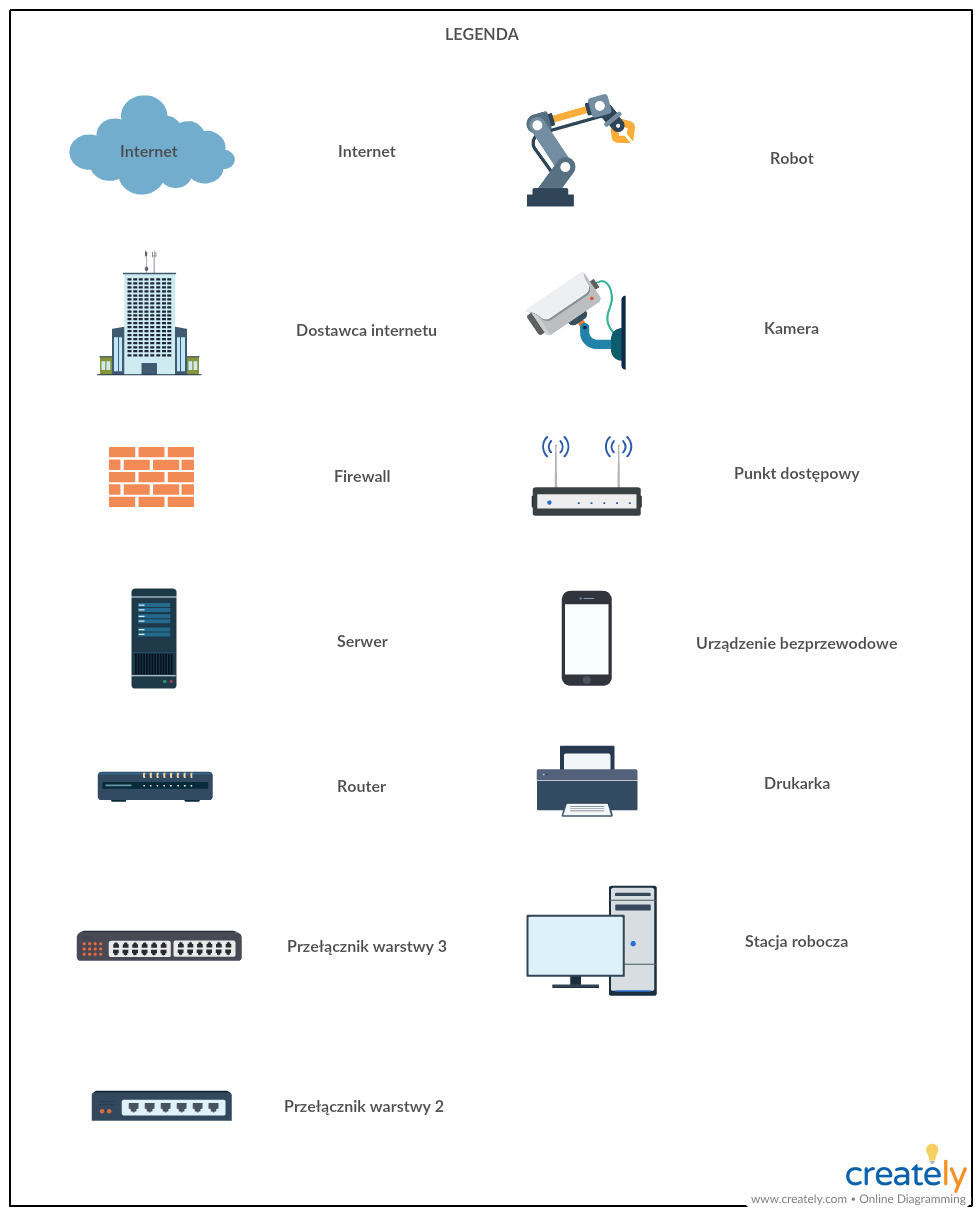
\includegraphics[width=14cm]{images/Legenda.png}
    \caption{Symbole użyte w logicznym projekcie sieci}
    \label{fig:Legenda}
\end{figure}

\newpage
\begin{figure}[H]
  \centering
    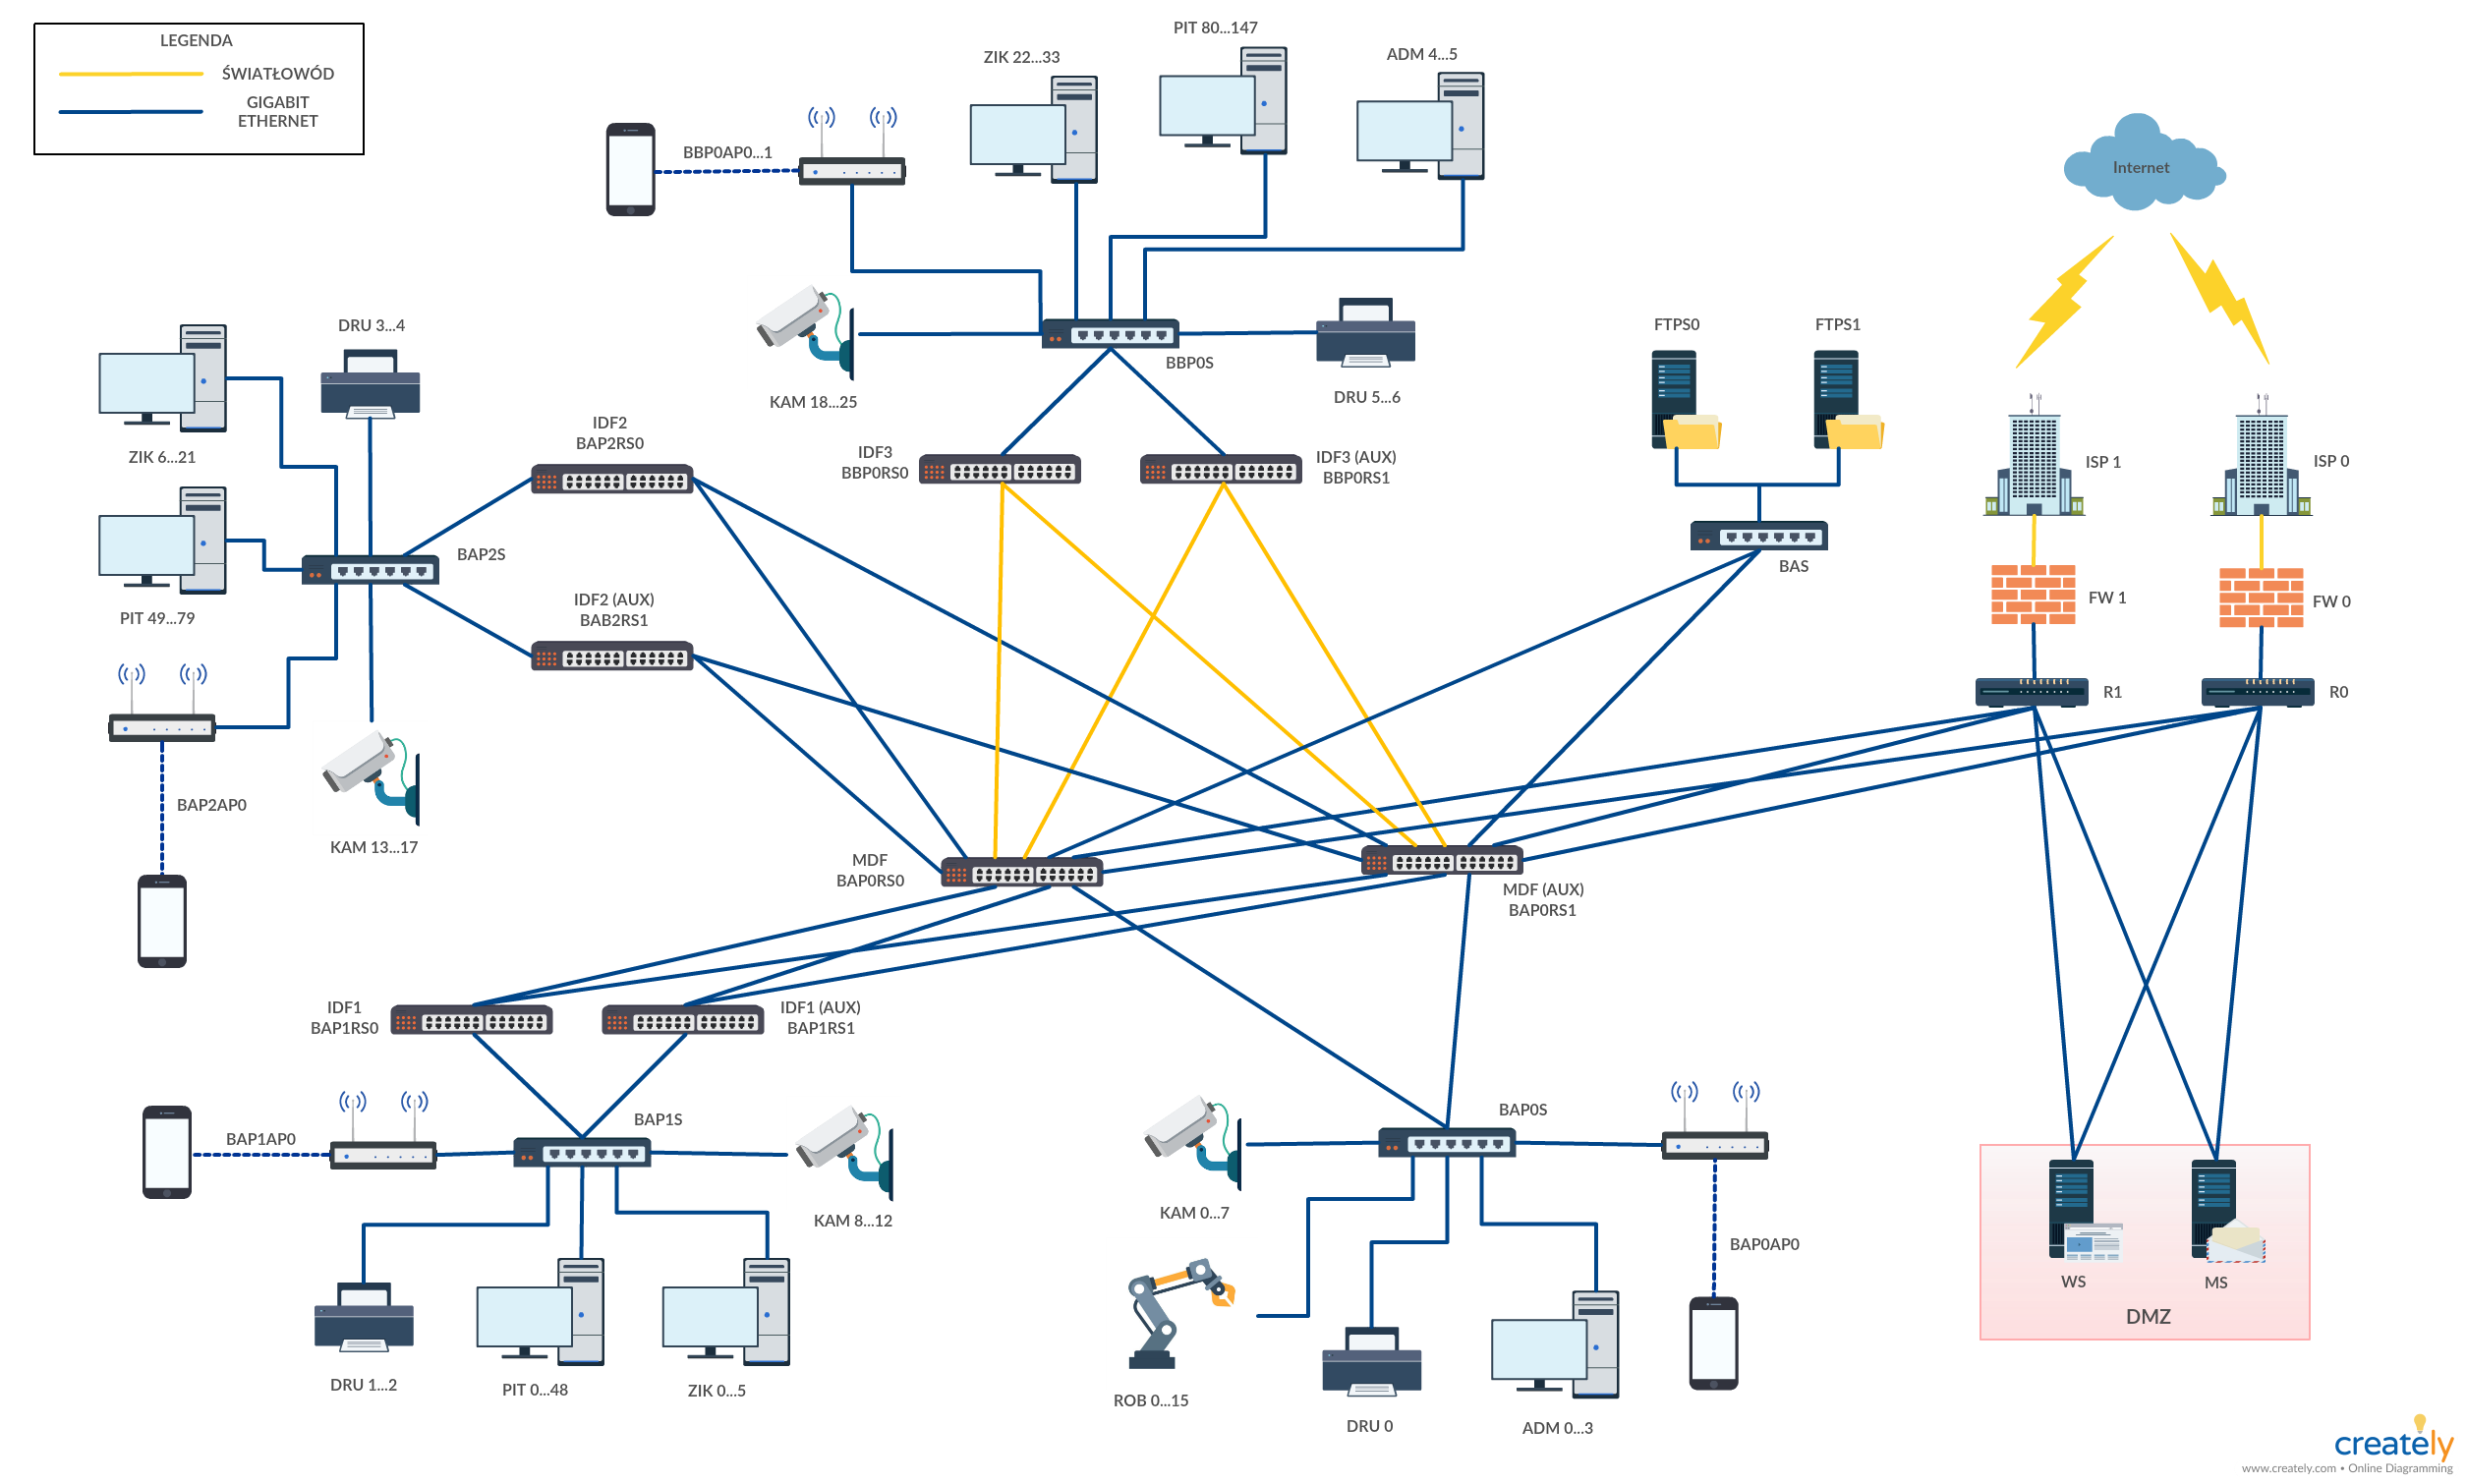
\includegraphics[height=14cm, angle=90]{images/Logical_diagram.png}
    \caption{Projekt logiczny sieci}
    \label{fig:Projekt}
\end{figure}

\newpage
\begin{figure}[H]
  \centering
    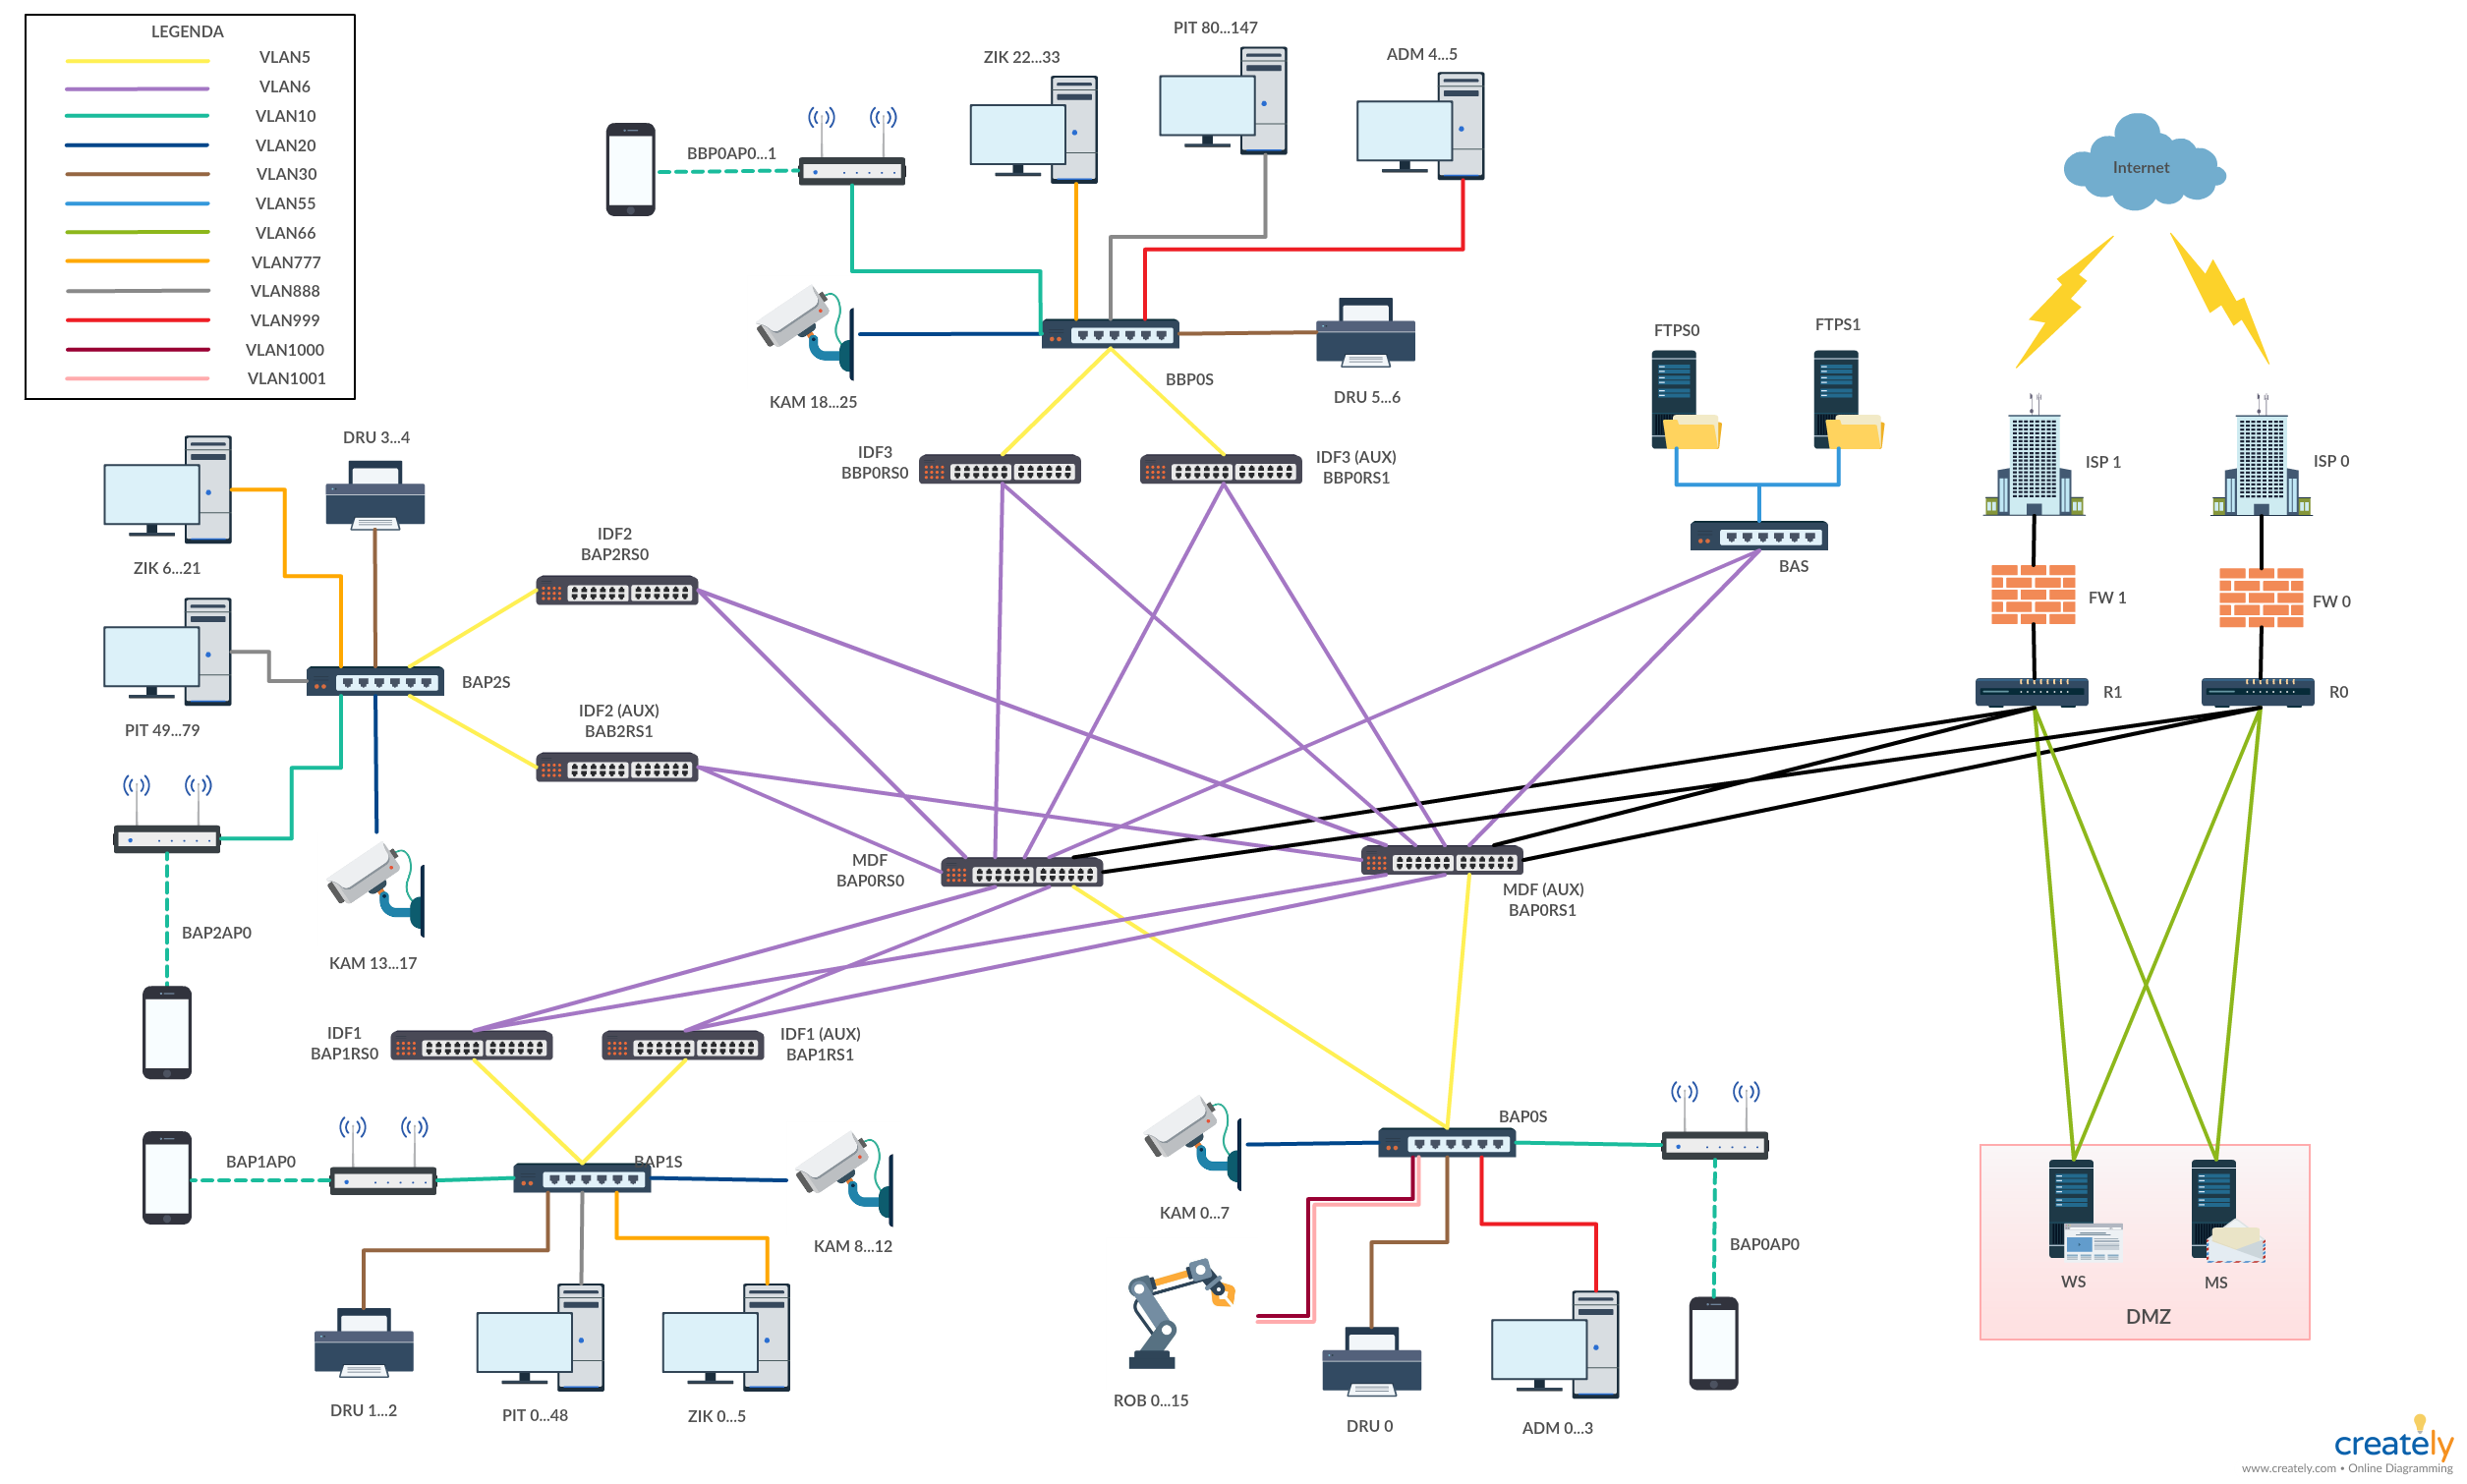
\includegraphics[height=14cm, angle=90]{images/Logical_diagram_VLAN.png}
    \caption{Podział VLAN}
    \label{fig:VLAN}
\end{figure}

\subsection{Urządzenia sieciowe}

\subsubsection{Przełączniki warstwy 3}
\begin{itemize}
    \item Producent: \textbf{CISCO}
    \item Model: \textbf{Catalyst 3650 48 Port PoE 4x1G Uplink LAN Base (WS-C3650-48PS-L)}
    \item Dodatkowe moduły:  CISCO SFP-10G-SR 10GBASE-SR SFP Module
\end{itemize}

Przełącznik ten posiada 48 portów Gigabit Ethernet. Wybraliśmy ten przełącznik gdyż ma możliwość
rozszerzenia go za pomocą modułów SFP. Po wyposażeniu go w moduł SFP-10G-SR można podłączyć
do łącza światłowodowego wielomodowego 10GBASE. Oprócz tego wspiera funkcje EtherChannel pozwalająca połączyć kilka łączy Ethernet w jedno logiczne. Duża liczba portów zapewni nam możliwość ewentualnej rozbudowy sieci w przyszłości.

\subsubsection{Przełączniki warstwy 2}
\begin{itemize}
    \item Producent: \textbf{CISCO}
    \item Model: \textbf{Catalyst 2960-X 48 GigE, 2 x 1G SFP, LAN Base (WS-C2960X-48TS-L)}
    \item Dodatkowe moduły: CISCO CATALYST 2960-X FLEXSTACK PLUS STACKING MODULE
\end{itemize}

Przełącznik posiada 48 portów Gigabit Ethernet. Głównym powodem wyboru tego przełącznika była potrzeba wykorzystania technologii FlexStack Plus. Przełącznik po wyposażeniu w dodatkowy moduł można połączyć razem z innymi przełącznikami firmy Cisco wspierającymi ta technologie (do 8
urządzeń). Urządzenia połączone w ten sposób zachowują się jak jedno logiczne urządzenie. Niesie to szereg zalet:

\begin{itemize}
    \item Uproszczone zarządzanie: wszystkie przełączniki są zarządzane jak jedno urządzenie. Dodatkowo są automatycznie aktualizowane kiedy główny przełącznik otrzymuje aktualizacje oprogramowania.
    \item W razie ewentualnej rozbudowy sieci po dołączeniu nowego przełącznika do stacku otrzymuje on automatycznie konfiguracje.
\end{itemize}

My użyjemy tej technologii aby uzyskać logiczny przełącznik posiadający 144 porty Gigabit Ethernet (3 przełączniki w stacku). Taka konfiguracja zostanie zastosowana na parterze budynku B. Na pozostałych piętrach zostanie zastosowana konfiguracja 2 przełączniki w stacku (96 portów). Pozwoli to na zapewnienie wolnych portów na przełącznikach (w liczbie 20\% zajętych portów). Przełącznik tego typu zostanie również użyty w pomieszczeniu z serwerami.

\subsubsection{Routery}
\begin{itemize}
    \item Producent: \textbf{CISCO}
    \item Model: \textbf{3945/K9 w/SPE150(3GE,4EHWIC,4DSP,4SM,256MBCF,1GBDRAM,IPB) (CISCO3945/
K9)}
    \item Dodatkowe moduły: Moduł Cisco mini-GBIC/SFP Gigabit 1000Base-T(RJ45) Module (MGBT1)
\end{itemize}

Router ten został wyposażony w 3 gniazda Gigabit Ethernet, posiada także 2 zainstalowane moduły SFP, 2 porty USB oraz port WAN. Po doposażeniu w moduły SFP Gigabit 1000Base-T otrzymamy wymagana ilość portów do obsługi naszej sieci. Wybraliśmy ten model ze względu na możliwość obsługi protokołu VRRP, a także obsługę standardu IEEE 802.3ab.

\subsubsection{Punkty dostępowe}
\begin{itemize}
    \item Producent: \textbf{CISCO}
    \item Model: \textbf{AIRONET 2702E DUAL BAND AP (AIR-CAP2702E-E-K9)}
\end{itemize}

Wybrany przez nas punkt dostępu obsługuje standardy IEEE 802.11a/b/g/n/ac. Zdecydowaliśmy się na ten model ze względu na obsługę dwóch pasm częstotliwości: 2,4GHz i 5GHz i duża prędkość
transmisji danych – 450 Mbps. Kolejna zaleta tego urządzenia jest gwarancja producenta trwająca do 5 lat od wycofania ze sprzedaży. Pozwoli to na bezproblemowe użytkowanie sprzętu, a w razie awarii zapewni naprawę lub wymianę na nowy.

\subsubsection{Zasilacz awaryjny}
\begin{itemize}
    \item Producent: \textbf{APC}
    \item Model: \textbf{Smart-UPS 2200VA LCD RM 2U 230V (SMT2200RMI2U)}
\end{itemize}
Zasilacz awaryjny Smart-UPS firmy APC to wysokiej klasy urządzenie w obudowie Rack 2U o mocy 2200VA/1980W. Urządzenie wyposażone jest w baterie ołowiowo-kwasowe (czas pełnego naładowania 3 godziny). Urządzenie wyposażono również w filtr napięcia chroniący podłączone obciążenia przed przepięciami, impulsami elektrycznymi, uderzeniami pioruna i innymi zakłóceniami zasilania. Ładowanie akumulatorów dostosowane jest do temperatury, dzięki czemu czas ich eksploatacji wydłuża się. Funkcja zimnego startu pozwala na tymczasowe zasilanie akumulatorowe w czasie zaniku zasilania sieciowego. Przy pełnym obciążeniu UPS jest w stanie podtrzymać napięcie na ok. 7 minut. W naszym przypadku użyjemy po 1 UPS-ie na każdy serwer oraz po jednym na każdy router. Pozwoli to w razie krótkotrwałej przerwy w dostawie energii elektrycznej utrzymać działanie serwerów WWW i FTP (dostarczać treści użytkownikom sieci Internet). W przypadku dłuższej awarii serwery te będą miały czas na bezpieczne wyłączenie się. W podobny sposób będzie to działało w przypadku serwerów sieci wewnętrznej. W celu redukcji kosztów zrezygnowaliśmy z podtrzymywania zasilania punktów dystrybucyjnych, gdyż w przypadku przerwy w dostawie zasilania stacje robocze nie będą działać (nie posiadają UPS-ów).

\subsection{Projekt adresacji IP} Sieć  zostanie  logicznie  podzielona  na  podsieci  odpowiadające  grupom  roboczymi pozostałym zaplanowanym VLAN-om. Wykorzystana zostanie adresacja prywatna–sieć 192.168.0.0/16, podzielona na podsieci o 24 bitowej masce oraz 30 bitowej masce dla sieci punkt-punkt. Adresem bramy domyślnej będzie zawsze pierwszy adres urządzenia dostępny w  danej  podsieci  tj.  192.168.X.1.Adresy  urządzeń  dostępowych  będą  przydzielane statycznie. Serwery lokalne, punkty dostępowe WiFi, przełączniki konfigurowalne, kamery oraz drukarki otrzymają adresy statyczne.\\
Przewidziane są następujące podsieci:
\begin{itemize}
    \item Grupa robocza "Zarząd i kadry"  -  VLAN777 - 192.168.1.0/24
    \item Grupa robocza "Programiści i testerzy"  -  VLAN888 - 192.168.2.0/24
    \item Grupa robocza "Administratorzy" -  VLAN999 - 192.168.3.0/24
    \item Sieć bezprzewodowa WiFi -  VLAN10 - 192.168.4.0/24
    \item Kamery  -  VLAN20 - 192.168.5.0/24
    \item Drukarki - VLAN30 - 192.168.6.0/24
    \item Serwery FTP  - VLAN55 - 192.168.7.0/24
    \item Roboty  -  VLAN1000 - 192.168.8.0/24
    \item Roboty (interfejs debugowania) - VLAN1001 - 192.168.255.0/24
    \item DMZ - VLAN66 - 192.168.9.0/24
    \item Przełączniki dostępowe - VLAN5 - 192.168.10.0/24
    \item Przełączniki szkieletowe - VLAN6 - 192.168.11.0/24
    
    
    \item Połączenie pomiędzy przełącznikiem szkieletowym BAP0RS0 a routerem\\R0 - 192.168.12.0/30
    \item Połączenie pomiędzy przełącznikiem szkieletowym BAP0RS0 a routerem\\R1 - 192.168.12.4/30
    \item Połączenie pomiędzy przełącznikiem szkieletowym BAP0RS1 a routerem\\R0 - 192.168.12.8/30
    \item Połączenie pomiędzy przełącznikiem szkieletowym BAP0RS1 a routerem\\R1 - 192.168.12.12/30
\end{itemize}

\newpage
\subsection{Projekt podłączenia do internetu}
    {\centering
    \small
    \begin{longtable}{|c|l|l|l|l|c|l|}
    \caption{Projekt podłączenia do internetu} \\
    \hline
    \textbf{Urządzenie} & \textbf{Interfejs} & \textbf{Połączenie} & \textbf{VLAN} & \textbf{Sieć} & \textbf{Maska} & \textbf{Adres} \\
    \hline
    \multirow{4}{*}{R0}
    & f0/0 & BAP0RS0 & - & 192.168.12.0 & /30 & 192.168.12.2 \\
    \cline{2-7}
    & f0/1 & BAP0RS1 & - & 192.168.12.8 & /30 & 192.168.12.10
 \\
    \cline{2-7}
    & f0/2 & MS & VLAN66 & 192.168.9.0 & /24 & 192.168.9.3
 \\
    \cline{2-7}
    & f0/3 & WS & VLAN66 & 192.168.9.0 & /24 & 192.168.9.5
 \\
    \hline
    
    \multirow{4}{*}{R1}
    & f0/0 & BAP0RS0 & - & 192.168.12.4 & /30 & 192.168.12.6
 \\
    \cline{2-7}
    & f0/1 & BAP0RS1 & - & 192.168.12.12 & /30 & 192.168.12.14
 \\
    \cline{2-7}
    & f0/2 & MS & VLAN66 & 192.168.9.0 & /24 & 192.168.9.7
 \\
    \cline{2-7}
    & f0/3 & WS & VLAN66 & 192.168.9.0 & /24 & 192.168.9.9
 \\
    \hline
    
    \multirow{10}{*}{BAP0RS0}
    & f0/0 & R0      & - & 192.168.12.0 & /30 & 192.168.12.3
 \\
    \cline{2-7}
    & f0/1 & R1      & - & 192.168.12.4 & /30 & 192.168.12.7
 \\
    \cline{2-7}
    & f0/2 & BAP0S   & VLAN5 & 192.168.10.0 & /24 & 192.168.10.3
 \\
    \cline{2-7}
    & f0/3 & BAP1RS0 & VLAN6  & 192.168.11.0 & /24 & 192.168.11.3
 \\
    \cline{2-7}
    & f0/4 & BAP1RS1 & VLAN6  & 192.168.11.0 & /24 & 192.168.11.5
 \\
    \cline{2-7}
    & f0/5 & BAP2RS0 & VLAN6  & 192.168.11.0 & /24 & 192.168.11.7
 \\
    \cline{2-7}
    & f0/6 & BAP2RS1 & VLAN6  & 192.168.11.0 & /24 & 192.168.11.9
 \\
    \cline{2-7}
    & f0/7 & BBP0RS0 & VLAN6  & 192.168.11.0 & /24 & 192.168.11.11
 \\
    \cline{2-7}
    & f0/8 & BBP0RS1 & VLAN6  & 192.168.11.0 & /24 & 192.168.11.13
 \\
    \cline{2-7}
    & f0/9 & BAS     & VLAN5 & 192.168.10.0 & /24 & 192.168.10.7
 \\
    \hline
    
    \multirow{10}{*}{BAP0RS1}
    & f0/0 & R0      & -  & 192.168.12.8 & /30 & 192.168.12.11
 \\
    \cline{2-7}
    & f0/1 & R1      & -  & 192.168.12.12 & /30 & 192.168.12.15
 \\
    \cline{2-7}
    & f0/2 & BAP0S   & VLAN5 & 192.168.10.0 & /24 & 192.168.10.5
 \\
    \cline{2-7}
    & f0/3 & BAP1RS0 & VLAN6  & 192.168.11.0 & /24 & 192.168.11.15
 \\
    \cline{2-7}
    & f0/4 & BAP1RS1 & VLAN6  & 192.168.11.0 & /24 & 192.168.11.17
 \\
    \cline{2-7}
    & f0/5 & BAP2RS0 & VLAN6  & 192.168.11.0 & /24 & 192.168.11.19
 \\
    \cline{2-7}
    & f0/6 & BAP2RS1 & VLAN6  & 192.168.11.0 & /24 & 192.168.11.21
 \\
    \cline{2-7}
    & f0/7 & BBP0RS0 & VLAN6  & 192.168.11.0 & /24 & 192.168.11.23
 \\
    \cline{2-7}
    & f0/8 & BBP0RS1 & VLAN6  & 192.168.11.0 & /24 & 192.168.11.25
 \\
    \cline{2-7}
    & f0/9 & BAS     & VLAN5 & 192.168.10.0 & /24 & 192.168.10.9
 \\
    \hline
    
    \multirow{3}{*}{BAP1RS0}
    & f0/0 & BAP1S & VLAN5 & 192.168.10.0 & /24 & 192.168.10.11
 \\
    \cline{2-7}
    & f0/1 & BAP0RS0 & VLAN6  & 192.168.11.0 & /24 & 192.168.11.2
 \\
    \cline{2-7}
    & f0/2 & BAP0RS1 & VLAN6  & 192.168.11.0 & /24 & 192.168.11.4
 \\
    \hline
    
    \multirow{3}{*}{BAP1RS1}
    & f0/0 & BAP1S & VLAN5 & 192.168.10.0 & /24 & 192.168.10.13
 \\
    \cline{2-7}
    & f0/1 & BAP0RS0 & VLAN6  & 192.168.11.0 & /24 & 192.168.11.6
 \\
    \cline{2-7}
    & f0/2 & BAP0RS1 & VLAN6  & 192.168.11.0 & /24 & 192.168.11.8
 \\
    \hline
    
    \multirow{3}{*}{BAP2RS0}
    & f0/0 & BAP2S & VLAN5 & 192.168.10.0 & /24 & 192.168.10.15
 \\
    \cline{2-7}
    & f0/1 & BAP0RS0 & VLAN6  & 192.168.11.0 & /24 & 192.168.11.10
 \\
    \cline{2-7}
    & f0/2 & BAP0RS1 & VLAN6  & 192.168.11.0 & /24 & 192.168.11.12
 \\
    \hline
    
    \multirow{3}{*}{BAP2RS1}
    & f0/0 & BAP2S & VLAN5 & 192.168.10.0 & /24 & 192.168.10.17
 \\
    \cline{2-7}
    & f0/1 & BAP0RS0 & VLAN6  & 192.168.11.0 & /24 & 192.168.11.14
 \\
    \cline{2-7}
    & f0/2 & BAP0RS1 & VLAN6  & 192.168.11.0 & /24 & 192.168.11.16
 \\
    \hline
    
    \multirow{3}{*}{BBP0RS0}
    & f0/0 & BBP0S & VLAN5 & 192.168.10.0 & /24 & 192.168.10.19
 \\
    \cline{2-7}
    & f0/1 & BAP0RS0 & VLAN6  & 192.168.11.0 & /24 & 192.168.11.18
 \\
    \cline{2-7}
    & f0/2 & BAP0RS1 & VLAN6  & 192.168.11.0 & /24 & 192.168.11.20
 \\
    \hline
    
    \multirow{3}{*}{BBP0RS1}
    & f0/0 & BBP0S & VLAN5 & 192.168.10.0 & /24 & 192.168.10.21
 \\
    \cline{2-7}
    & f0/1 & BAP0RS0 & VLAN6 & 192.168.11.0 & /24 & 192.168.11.22
 \\
    \cline{2-7}
    & f0/2 & BAP0RS1 & VLAN6  & 192.168.11.0 & /24 & 192.168.11.24
 \\
    \hline
    
    \multirow{4}{*}{BAS}
    & f0/0 & BAP0RS0 & VLAN5 & 192.168.10.0 & /24 & 192.168.10.6
 \\
    \cline{2-7}
    & f0/1 & BAP0RS1 & VLAN5 & 192.168.10.0 & /24 & 192.168.10.10
 \\
    \cline{2-7}
    & f0/2 & FTPS0 & VLAN55 & 192.168.7.0 & /24 & 192.168.7.3
 \\
    \cline{2-7}
    & f0/3 & FTPS1 & VLAN55 & 192.168.7.0 & /24 & 192.168.7.5
 \\
    \hline
    
    \multirow{8}{*}{BAP0S}
    & f0/0 & BAP0RS0 & VLAN5 & 192.168.10.0 & /24 & 192.168.10.2
 \\
    \cline{2-7}
    & f0/1 & BAP0RS1 & VLAN5 & 192.168.10.0 & /24 & 192.168.10.4
 \\
    \cline{2-7}
    & f0/2 & BAP0AP0 & VLAN10 & 192.168.4.0 & /24 & 192.168.4.3
 \\
    \cline{2-7}
    & f0/3-10 & KAM0…7 & VLAN20 & 192.168.5.0 & /24 & 192.168.5.3-10
 \\
    \cline{2-7}
    & f0/11 & DRU0 & VLAN30 & 192.168.6.0 & /24 & 192.168.6.3
 \\
    \cline{2-7}
    & f0/12-15 & ADM0…3 & VLAN999 & 192.168.3.0 & /24 & 192.168.3.3-6
 \\
    \cline{2-7}
    & f0/16-31 & ROB0…15 & VLAN1000 & 192.168.8.0 & /24 & 192.168.8.3-18
 \\
    \cline{2-7}
    & f0/32-47 & ROB0…15 & VLAN1001 & 192.168.255.0 & /24 & 192.168.255.100 \\
    \hline
    
    \multirow{7}{*}{BAP1S}
    & f0/0 & BAP1RS0 & VLAN5 & 192.168.10.0 & /24 & 192.168.10.12
\\
    \cline{2-7}
    & f0/1 & BAP1RS1 & VLAN5 & 192.168.10.0 & /24 & 192.168.10.14
 \\
    \cline{2-7}
    & f0/2 & BAP1AP0 & VLAN10 & 192.168.4.0 & /24 & 192.168.4.4
 \\
    \cline{2-7}
    & f0/3-7 & KAM8…12 & VLAN20 & 192.168.5.0 & /24 & 192.168.11-15
 \\
    \cline{2-7}
    & f0/8-9 & DRU1…2 & VLAN30 & 192.168.6.0 & /24 & 192.168.6.5-6
 \\
    \cline{2-7}
    & f0/10-15 & ZIK0…5 & VLAN777 & 192.168.1.0 & /24 & 192.168.1.3-8
 \\
    \cline{2-7}
    & f0/16-64 & PIT0…48 & VLAN888 & 192.168.2.0 & /24 & 192.168.2.3-51
 \\
    \hline
    
    \multirow{7}{*}{BAP2S}
    & f0/0 & BAP2RS0 & VLAN5 & 192.168.10.0 & /24 & 192.168.10.16
 \\
    \cline{2-7}
    & f0/1 & BAP2RS1 & VLAN5 & 192.168.10.0 & /24 & 192.168.10.18
 \\
    \cline{2-7}
    & f0/2 & BAP2AP0 & VLAN10 & 192.168.4.0 & /24 & 192.168.4.5
 \\
    \cline{2-7}
    & f0/3-7 & KAM13…17 & VLAN20 & 192.168.5.0 & /24 & 192.168.5.16-20
 \\
    \cline{2-7}
    & f0/8-9 & DRU3…4 & VLAN30 & 192.168.6.0 & /24 & 192.168.6.6-7
 \\
    \cline{2-7}
    & f0/10-25 & ZIK6…21 & VLAN777 & 192.168.1.0 & /24 & 192.168.1.9-24
 \\
    \cline{2-7}
    & f0/26-56 & PIT49…79 & VLAN888 & 192.168.2.0 & /24 & 192.168.2.52-82
 \\
    \hline
    
    \multirow{8}{*}{BBP0S}
    & f0/0 & BBP0RS0 & VLAN5 & 192.168.10.0 & /24 & 192.168.10.20
 \\
    \cline{2-7}
    & f0/1 & BBP0RS1 & VLAN5 & 192.168.10.0 & /24 & 192.168.10.22
 \\
    \cline{2-7}
    & f0/2 & BBP0AP0…1 & VLAN10 & 192.168.4.0 & /24 & 192.168.4.6-7
 \\
    \cline{2-7}
    & f0/3-10 & KAM18…25 & VLAN20 & 192.168.5.0 & /24 & 192.168.6.21-28
\\
    \cline{2-7}
    & f0/11-12 & DRU5…6 & VLAN30 & 192.168.6.0 & /24 & 192.168.6.8-9
 \\
    \cline{2-7}
    & f0/13-24 & ZIK22…33 & VLAN777 & 192.168.1.0 & /24 & 192.168.1.25-36
 \\
    \cline{2-7}
    & f0/25-92 & PIT80…147 & VLAN888 & 192.168.2.0 & /24 & 192.168.2.83-150
 \\
    \cline{2-7}
    & f0/93-94 & ADM4…5 & VLAN999 & 192.168.3.0 & /24 & 192.168.3.7-8
 \\
    \hline
\end{longtable}}

\newpage
\subsection{Analiza bezpieczeństwa i niezawodności sieci}

Oprogramowanie używane na stanowiskach komputerowych oraz odpowiednie zabezpieczenie komputerów leży po stronie zleceniodawcy. Podstawowa ochronę przeciwko atakom z zewnątrz zapewni odpowiednio skonfigurowana funkcja Cisco IOS Firewall na routerach. Ponadto:

\begin{itemize}
    \item Każde stanowisko komputerowe wymaga autoryzacji w sieci oraz na dedykowanym do tego serwerze,
    \item Połączenie z siecią bezprzewodową do zasobów sieci lokalnej wymaga autoryzacji na serwerze RADIUS oraz zabezpieczenia kluczem WPA2 Enterprise,
    \item Przewiduje się regularne szkolenia w zakresie podstawowej wiedzy bezpieczeństwa sieciowego oraz udostępniania danych wrażliwych,
    \item Pomieszczenia sieciowe zaopatrzone zostaną w odpowiednie centrale alarmowe oraz zamki szyfrowe, a każda ingerencja oraz dostęp do tych pomieszczeń skutkuje powiadomienie za pośrednictwem SMS/CLIP operatora lub właściciela oddziału,
    \item Bezpieczeństwo urządzeń sieciowych tj. przełączników, routerów sprowadza się do wyłączenia nieużywanych interfejsów sieciowych.
    \item Dane wrażliwe zapisywane oraz kodowane na specjalnych systemach back-up zarówno na dyskach twardych jak i na wymiennych nośnikach magnetycznych,
    \item Osoba upoważniona do nadzoru nad siecią teleinformatyczną jest zobowiązana do  opracowania polityki bezpieczeństwa uwzględniającej wyżej wymienione podpunkty,
    \item Pomieszczenie teletechniczne (serwerownia) znajduje się w osobnym pomieszczeniu, gdzie zostaną umieszczone wszystkie urządzenia sieciowe, tj.:
        \begin{itemize}
            \item Przełączniki,
            \item Routery,
            \item Systemy zasilania awaryjnego pozwalające na pracę urządzeń przez minimalny potrzebny czas do bezpiecznego wyłączenia i zarchiwizowania otwartych sesji sieciowych w przypadku awarii zasilania,
            \item Systemu krosownic, prowadnic kabli, torów kablowych, okablowania,
            \item Systemów nadzorowanego dostępu tzw. UTM oraz Firewall,
        \end{itemize}
    \item Zapewniona zostanie niezbędna redundancja oraz skalowalności sieci.
\end{itemize}
\subsection{Kosztorys}

\begin{table}[H]
    \caption{Kosztorys urządzeń}
    \centering
    \begin{tabular}{|c|c|c|c|}
    \hline
    \textbf{Urządzenie} & \specialcellbold{Cena za sztukę\\(netto)} & \textbf{Liczba} & \textbf{Cena łączna} \\
    \hline
    \specialcell{Cisco Catalyst 3650 48 Port\\PoE 4x1G Uplink LAN Base} & 15 639,34 zł & 8 & 125 114,72 zł \\
    \hline
    \specialcell{Cisco SFP-10G-SR\\10GBASE-SR SFP Module} & 1 265,47 zł & 8 & 10 123,76 zł \\
    \hline
    \specialcell{Cisco Catalyst 2960-X 48 GigE\\ 2 x 1G SFP LAN Base} & 5 373,78 zł & 10 & 53 737,80 zł \\
    \hline
    \specialcell{Cisco Catalyst 2960-X\\Flexstack-Plus Stack Module} & 2 158,69 zł & 9 & 19 428,21 zł \\
    \hline
    Cisco 3945/K9 & 31 025,43 zł & 2 & 62 050,86 zł \\
    \hline
    \specialcell{Cisco MGBT1 GbE 1000Base-T\\Mini-GBIC SFP Transceiver} & 377,68 zł & 2 & 755,36 zł \\
    \hline
    \specialcell{Cisco AIRONET 2702E\\DUAL BAND AP} & 1 754,96 zł & 5 & 8 774,8 zł \\
    \hline
    \specialcell{APC Smart-UPS 2200VA\\LCD RM 2U 230V} & 4 802,87 zł & 6 & 28 817,22 zł \\
    \hline
    \multicolumn{2}{c|}{} & \textbf{Razem} & \textbf{308 802,73 zł} \\
    \cline{3-4}
    \end{tabular}
    \label{tab:kosztorys}
\end{table}
\newpage
\section{Karty katalogowe proponowanych urządzeń}
\subsection{Przełączniki warstwy 3}
\textbf{Cisco Catalyst 3650 48 Port PoE 4x1G Uplink LAN Base}
\begin{itemize}
    \item \textbf{Model:} WS-C3650-48PS-L,
    \item \textbf{Ilość slotów w szafie montażowej:} 1U,
    \item \textbf{Liczba portów:} 48 10/100/1000 Ethernet PoE+,
    \item \textbf{Ilość pamięci Flash:} 2GB,
    \item \textbf{Ilość pamięci DRAM:} 4GB,
    \item \textbf{Dokładna specyfikacja:}  \url{https://www.cisco.com/c/en/us/products/collateral/switches/catalyst-3650-series-switches/data_sheet-c78-729449.html}
\end{itemize}
\begin{figure}[H]
  \centering
    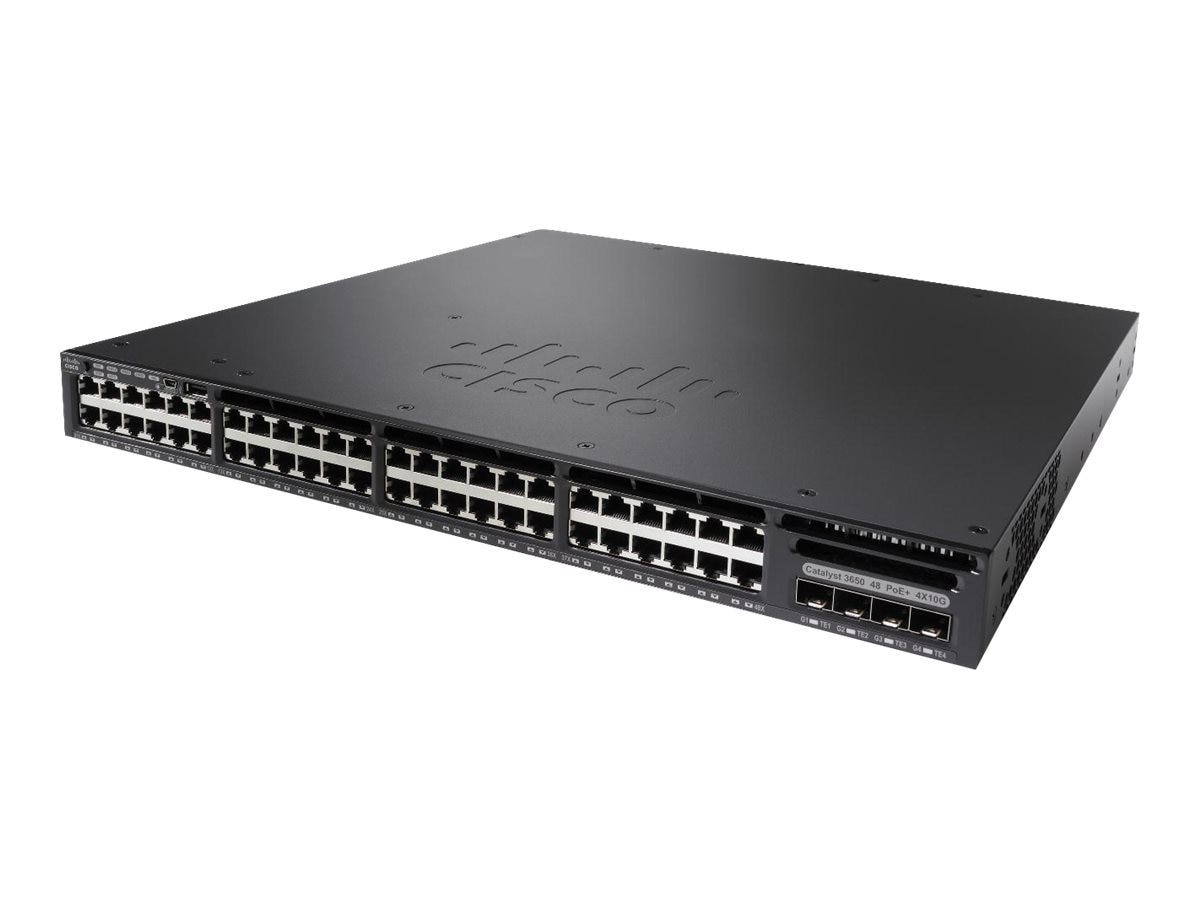
\includegraphics[width=14cm]{images/switch3.jpg}
    \caption{Cisco Catalyst 3650 48 Port PoE 4x1G Uplink LAN Base}
    \label{fig:switch3}
\end{figure}

\newpage
\subsection{Przełączniki warstwy 2}
\textbf{Cisco Catalyst 2960-X 48 GigE, 2 x 1G SFP, LAN Base}
\begin{itemize}
    \item \textbf{Model:} WS-C2960X-48TS-L,
    \item \textbf{Ilość slotów w szafie montażowej:} 1U,
    \item \textbf{Liczba portów:} 48 10/100/1000 Ethernet,
    \item \textbf{Ilość pamięci Flash:} 128MB,
    \item \textbf{Ilość pamięci DRAM:} 512MB,
    \item \textbf{Dokładna specyfikacja:}  \url{https://www.cisco.com/c/en/us/products/collateral/switches/catalyst-2960-x-series-switches/datasheet_c78-728232.html}
\end{itemize}
\begin{figure}[H]
  \centering
    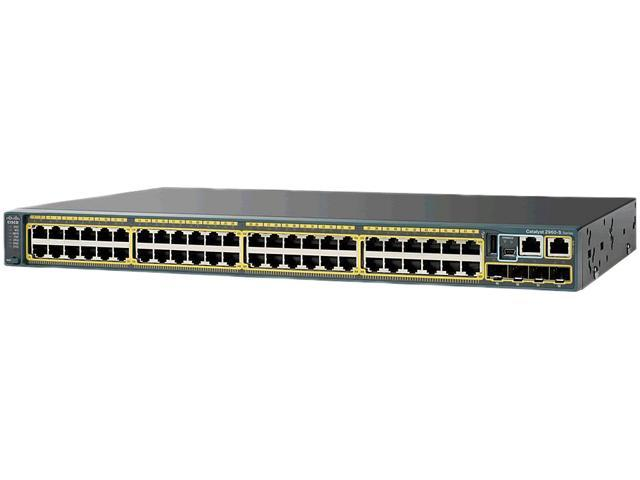
\includegraphics[width=14cm]{images/switch2.jpg}
    \caption{Cisco Catalyst 2960-X 48 GigE, 2 x 1G SFP, LAN Base}
    \label{fig:switch2}
\end{figure}

\newpage
\subsection{Routery}
\textbf{Cisco 3945/K9 w/SPE150(3GE,4EHWIC,4DSP,4SM,256MBCF,1GBDRAM,IPB)}
\begin{itemize}
    \item \textbf{Model:} CISCO3945/K9,
    \item \textbf{Ilość slotów w szafie montażowej:} 3U,
    \item \textbf{Liczba portów:} 3 10/100/1000 Ethernet,
    \item \textbf{Ilość pamięci Flash:} 256MB,
    \item \textbf{Ilość pamięci DRAM:} 1GB,
    \item \textbf{Dokładna specyfikacja:}  \url{https://www.cisco.com/c/en/us/products/collateral/routers/3900-series-integrated-services-routers-isr/data_sheet_c78_553924.html}
\end{itemize}
\begin{figure}[H]
  \centering
    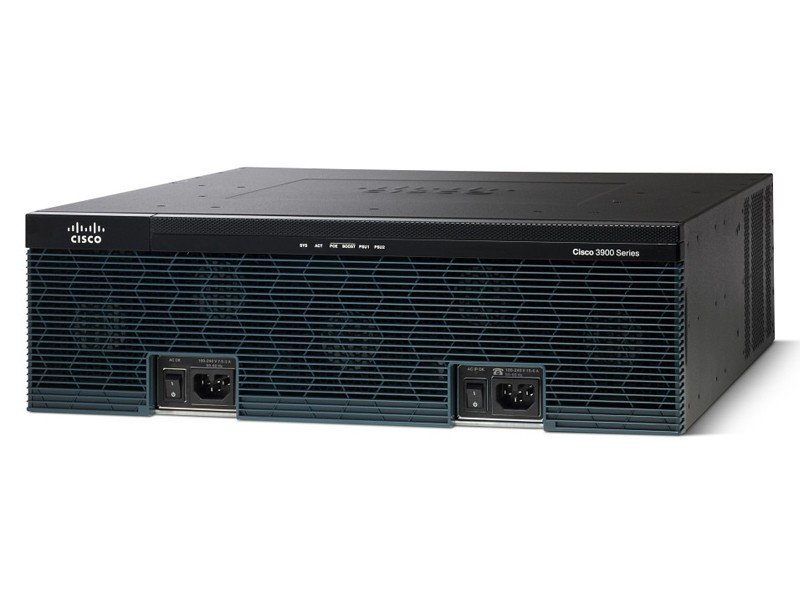
\includegraphics[width=14cm]{images/router.jpg}
    \caption{Cisco 3945/K9 w/SPE150}
    \label{fig:router}
\end{figure}

\newpage
\subsection{Punkty dostępowe}
\textbf{Cisco AIRONET 2702E DUAL BAND AP}
\begin{itemize}
    \item \textbf{Model:} AIR-CAP2702E-E-K9,
    \item \textbf{Ilość pamięci Flash:} 64MB,
    \item \textbf{Ilość pamięci DRAM:} 512MB,
    \item \textbf{Obsługiwane standardy:} IEEE 802.11b, IEEE 802.11a, IEEE 802.11g, IEEE 802.11n, IEEE 802.11ac
    \item \textbf{Pasmo częstotliwości:} 2.4GHz, 5GHz,  
    \item \textbf{Dokładna specyfikacja:} \url{https://www.cisco.com/c/en/us/products/collateral/wireless/aironet-2700-series-access-point/datasheet-c78-730593.html}
\end{itemize}
\begin{figure}[H]
  \centering
    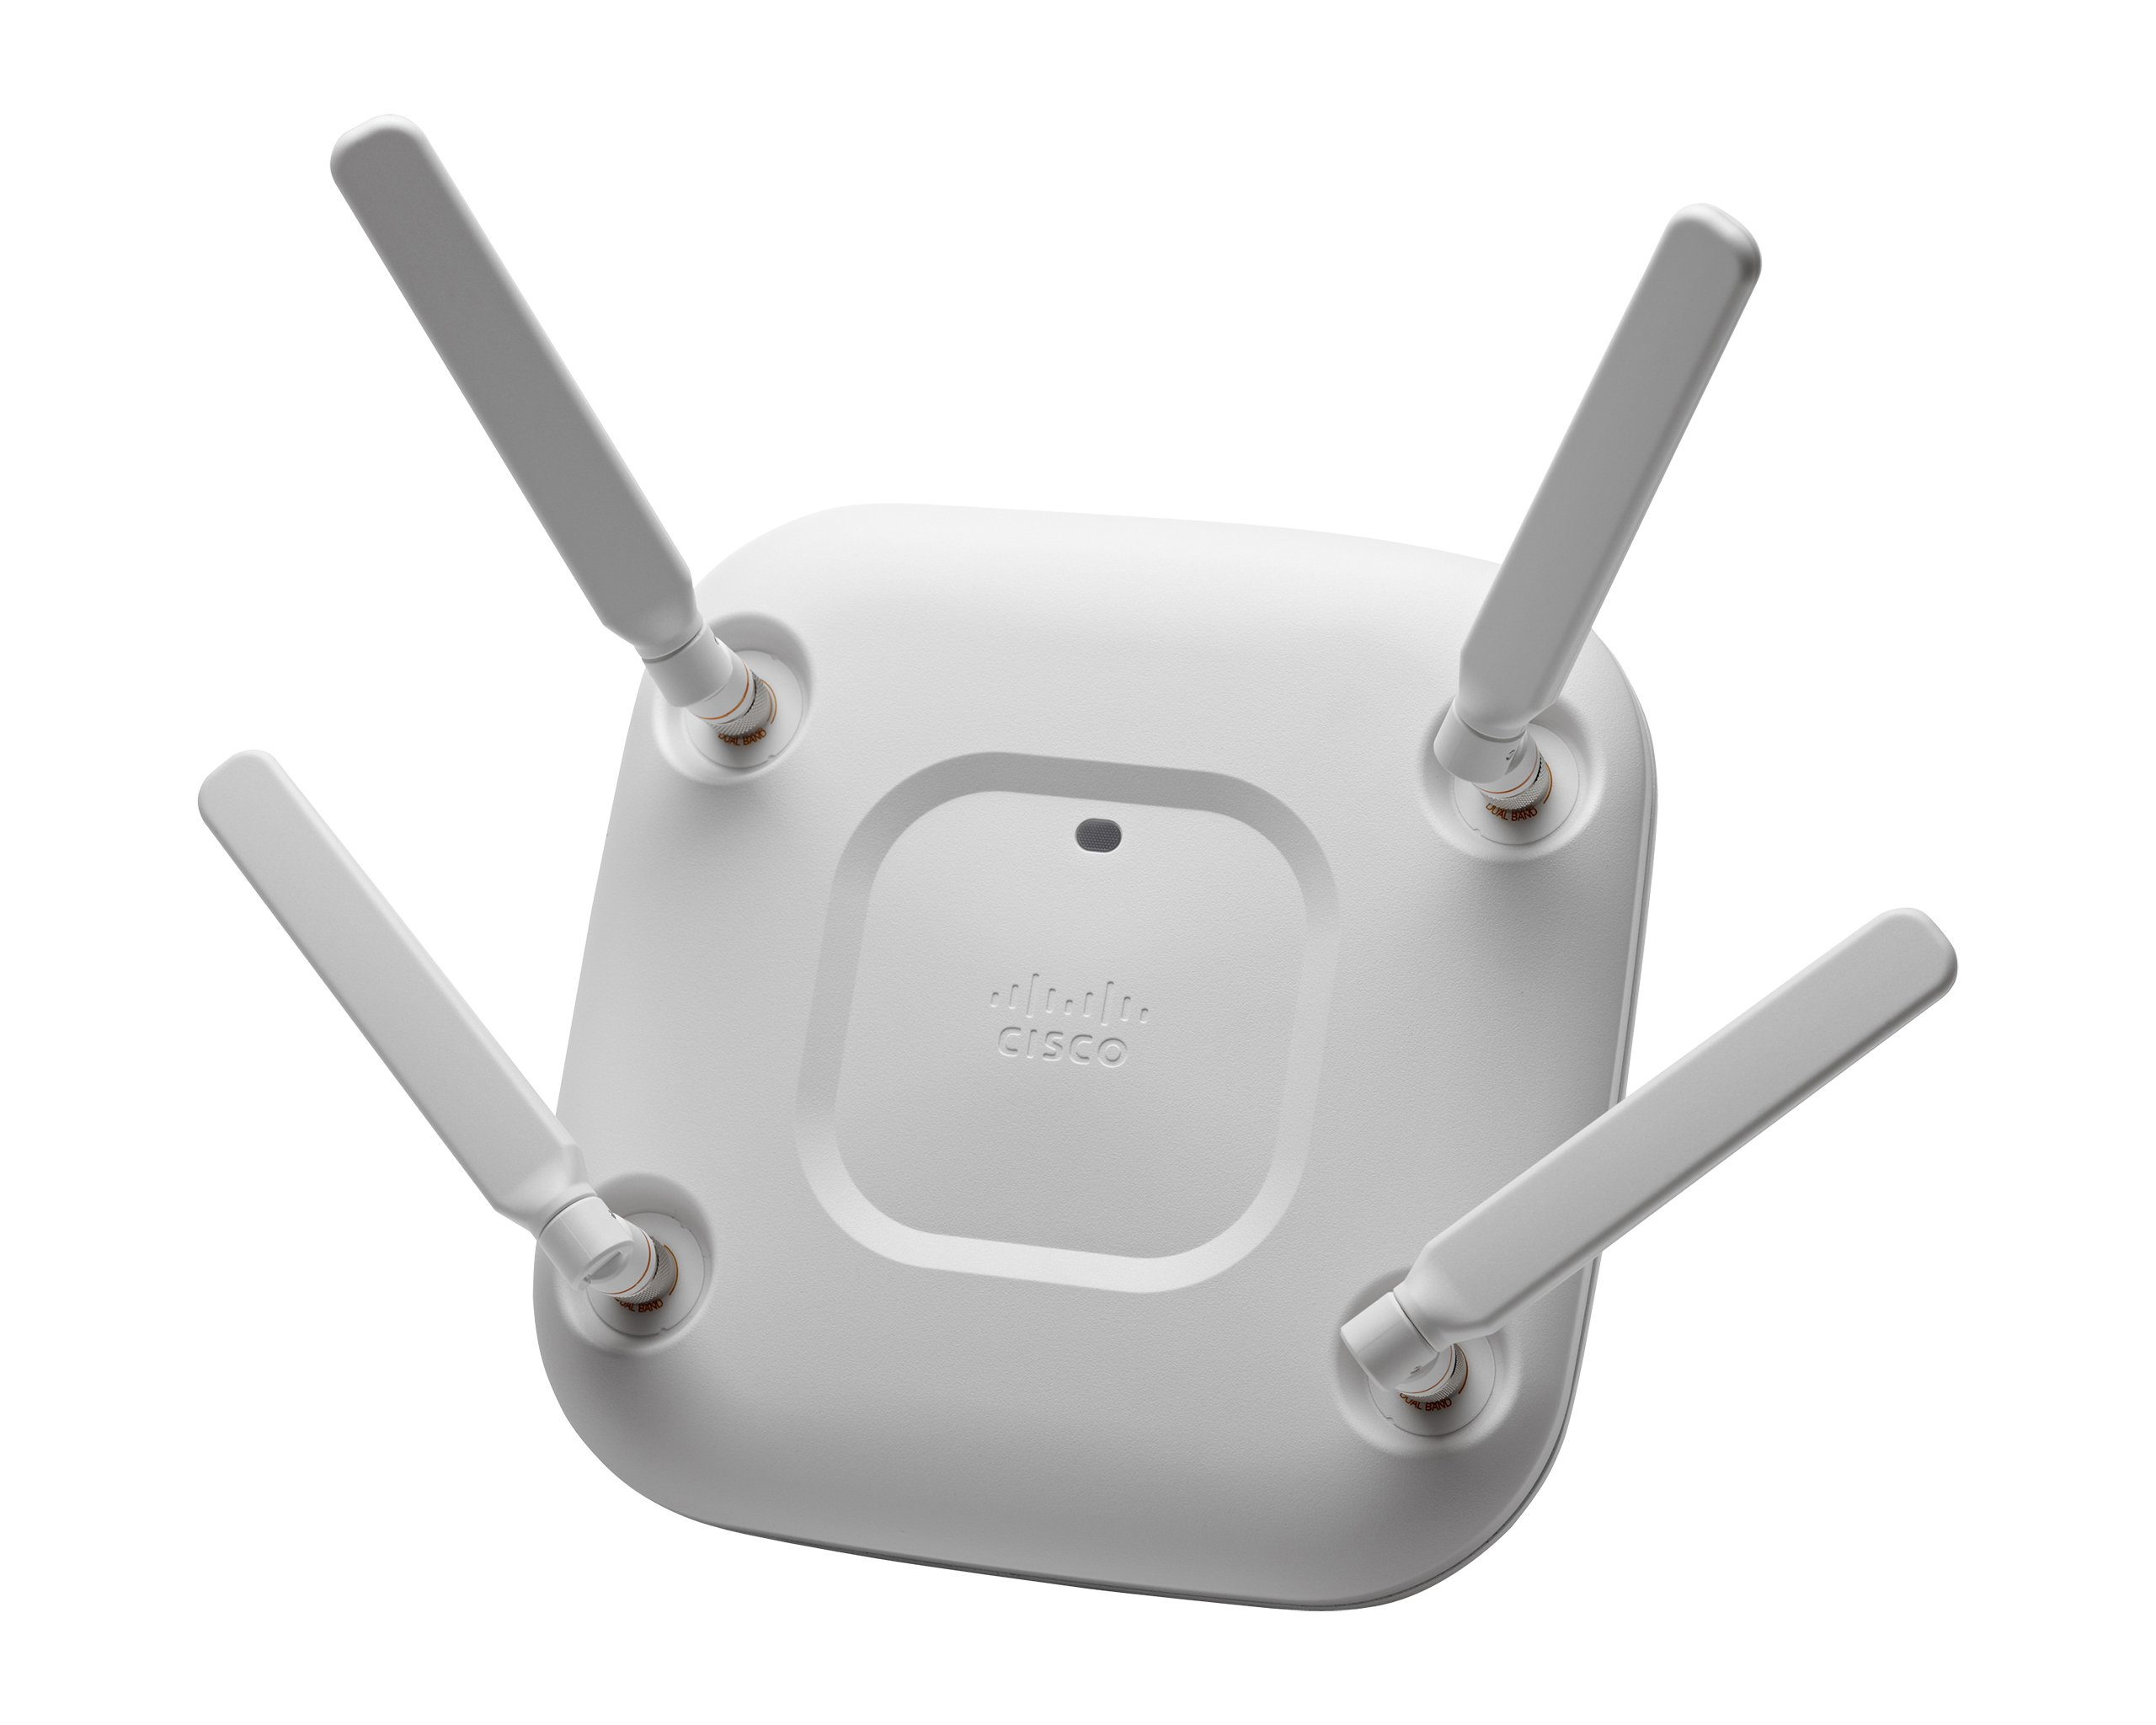
\includegraphics[width=14cm]{images/ap.jpg}
    \caption{Cisco AIRONET 2702E DUAL BAND AP}
    \label{fig:ap}
\end{figure}

\newpage
\subsection{Zasilacz awaryjny}
\textbf{APC Smart-UPS 2200VA LCD RM 2U 230V}
\begin{itemize}
    \item \textbf{Model:} SMT2200RMI2U,
    \item \textbf{Ilość slotów w szafie montażowej:} 3U,
    \item \textbf{Oczekiwana żywotność baterii:} 3-5 lat,
    \item \textbf{Nominalne napięcie wyjściowe:} 230V,
    \item \textbf{Moc wyjściowa:} 1.98KWatts/2.2kVA
    \item \textbf{Dokładna specyfikacja:} \url{https://www.cisco.com/c/en/us/products/collateral/wireless/aironet-2700-series-access-point/datasheet-c78-730593.html}
\end{itemize}
\begin{figure}[H]
  \centering
    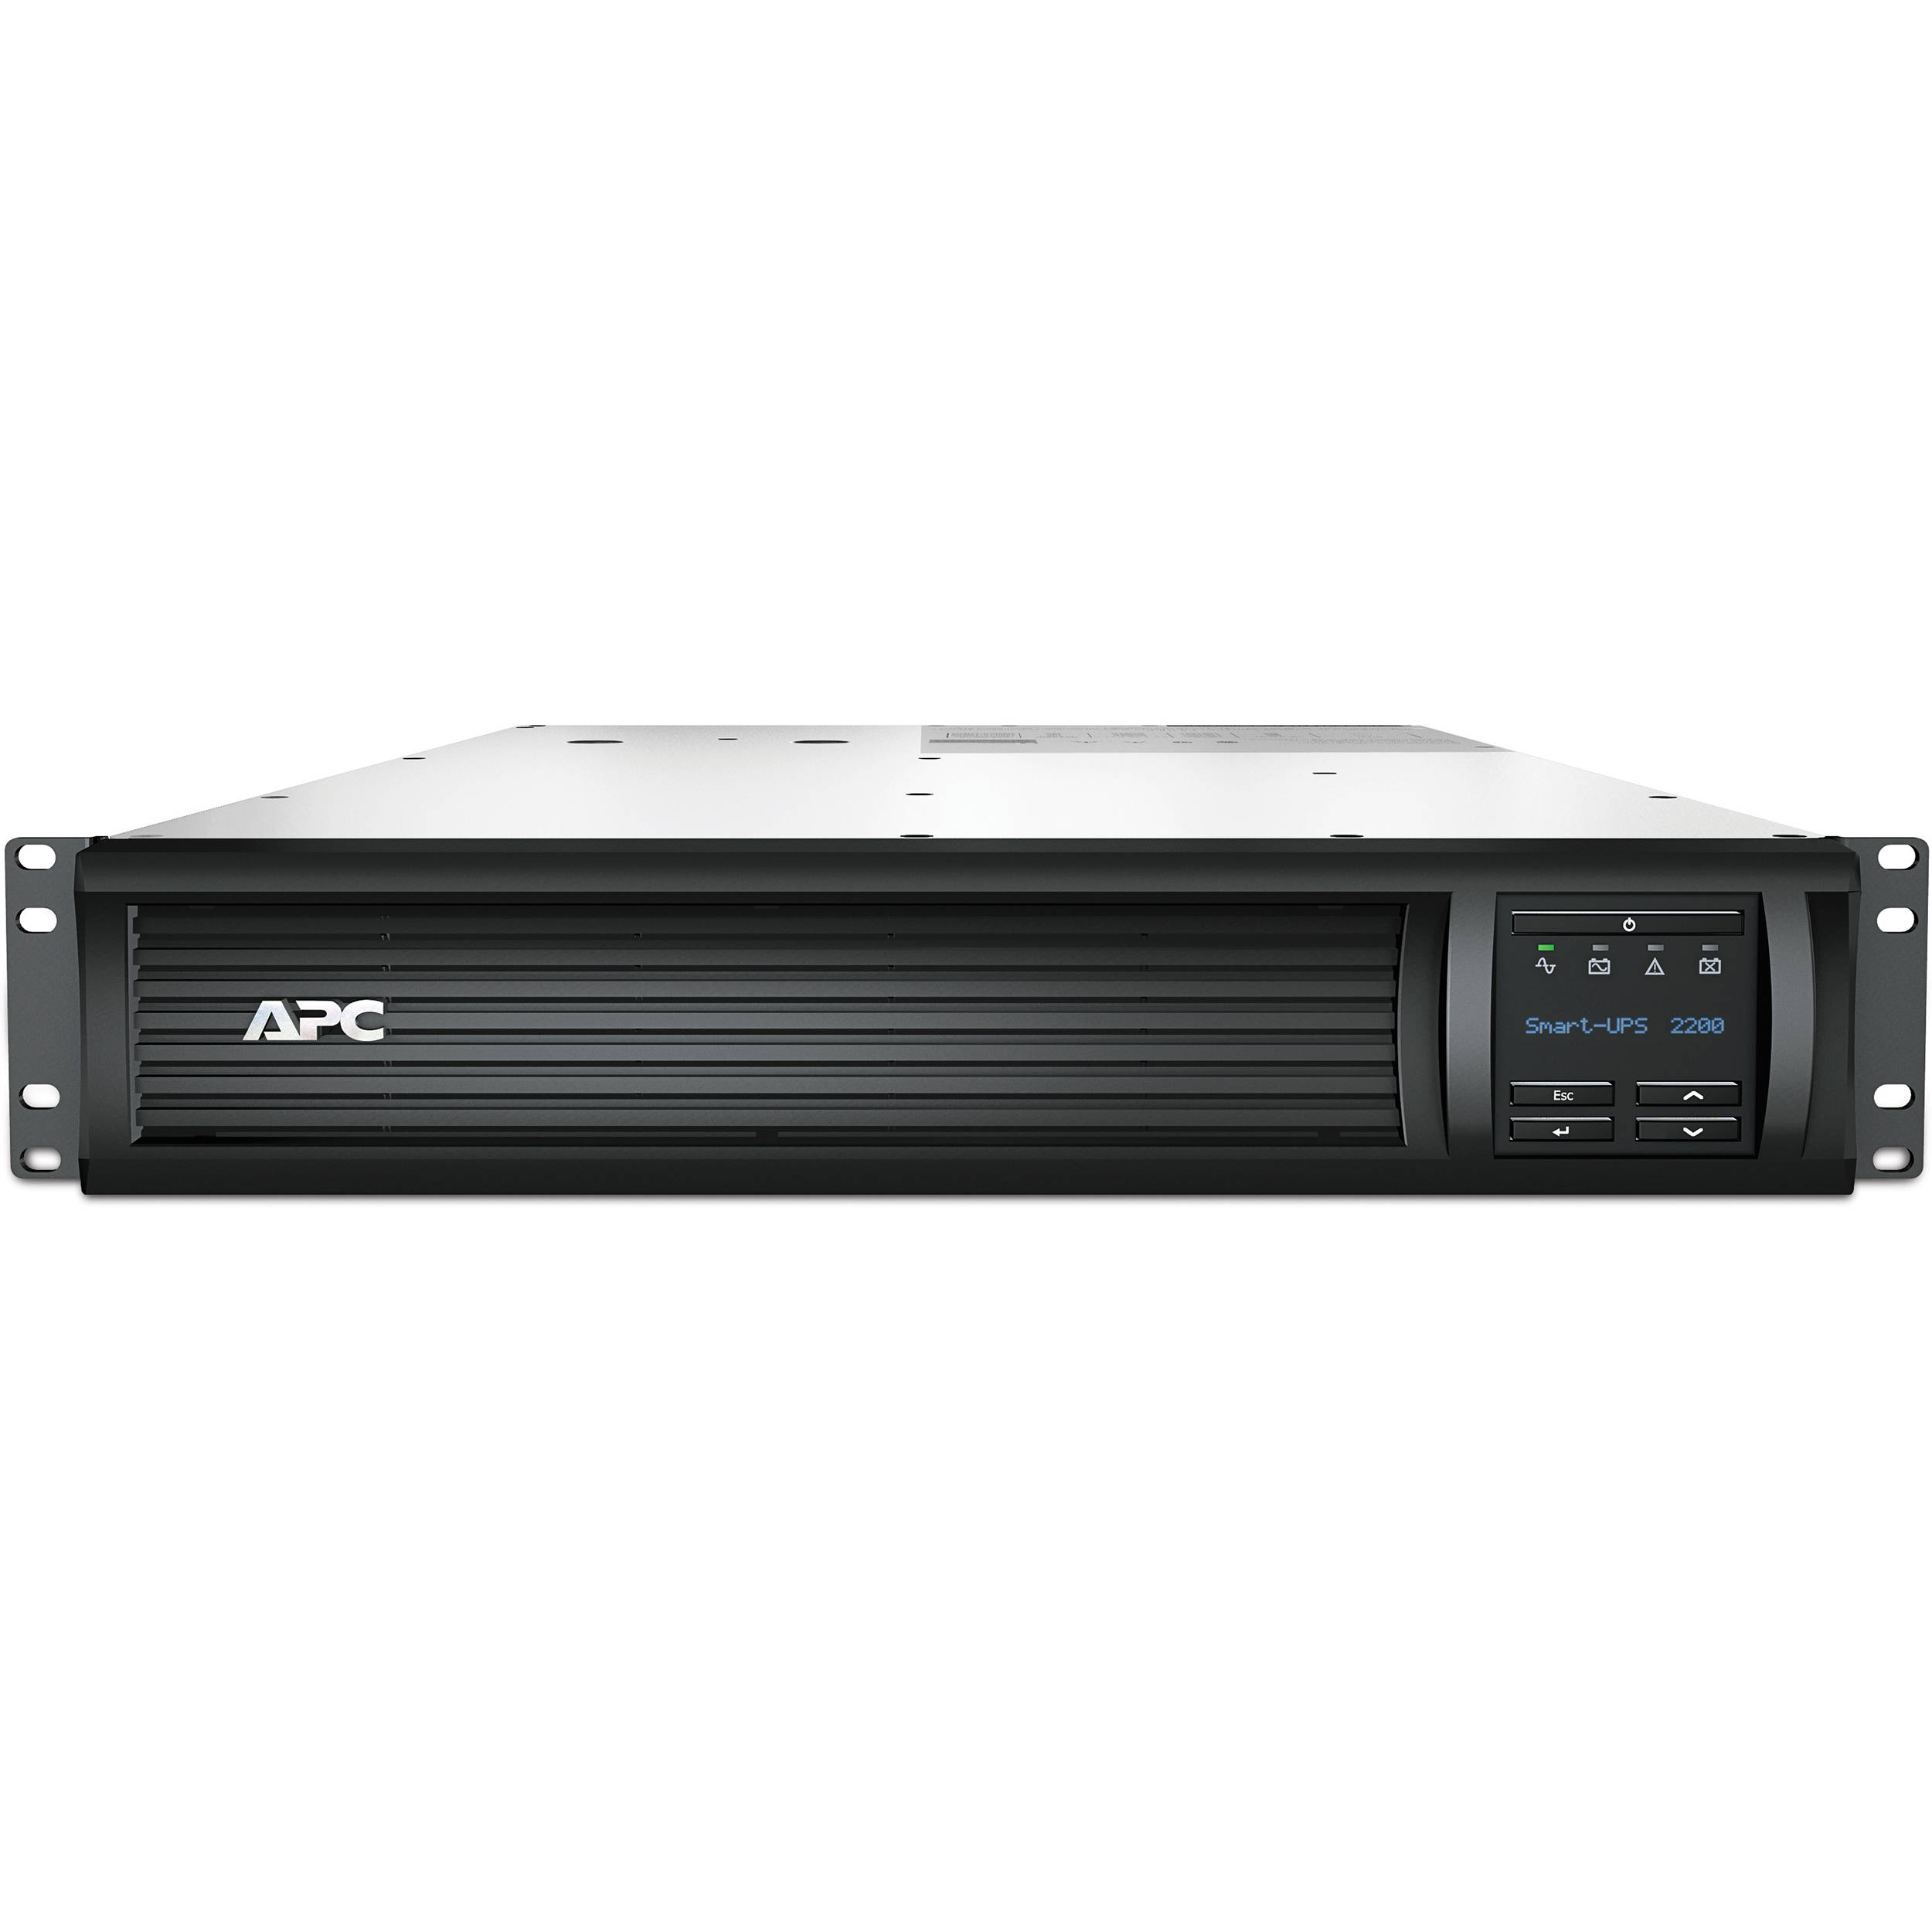
\includegraphics[width=14cm]{images/ups.jpg}
    \caption{APC Smart-UPS 2200VA LCD RM 2U 230V}
    \label{fig:ups}
\end{figure}

\newpage
\listoftables
\listoffigures
\end{document}